\documentclass[12pt,oneside]{book}

\usepackage{ulamonog} %proyecto de grado
\usepackage[utf8]{inputenc}

\usepackage{longtable}


% Para texto en chino, japonés o coreano:
\usepackage{CJKutf8}

% Para imágenes, tablas más agradables visualmente y listas de chequeo en tablas:
\usepackage{booktabs}%
\usepackage{graphicx}%
\graphicspath{ {img/} }
\usepackage{float}
\usepackage{pifont}% http://ctan.org/pkg/pifont
\usepackage[flushleft]{threeparttable}
\usepackage{adjustbox}
\newcommand{\cmark}{\ding{51}}%
\newcommand{\xmark}{\ding{55}}%

% Para mostrar código fuente:
\usepackage{textcomp}
\usepackage{listings}
\lstset{
basicstyle=\small\ttfamily,
columns=flexible,
breaklines=true,
upquote=true,
showstringspaces=false
}

% Para mostrar cuadros de información/advertencias:
\usepackage{xcolor}
\usepackage[tikz]{bclogo}
\usepackage[framemethod=tikz]{mdframed}
\usepackage[many]{tcolorbox}

\definecolor{bgblue}{RGB}{245,243,253}
\definecolor{ttblue}{RGB}{91,194,224}
\definecolor{electricyellow}{rgb}{1.0, 1.0, 0.0}

\mdfdefinestyle{mystyle}{%
  rightline=true,
  innerleftmargin=10,
  innerrightmargin=10,
  outerlinewidth=3pt,
  topline=false,
  rightline=true,
  bottomline=false,
  skipabove=\topsep,
  skipbelow=\topsep
}

\newtcolorbox{blackcodebox}[1][]{
  breakable,
  title=#1,
  colback=white,
  colbacktitle=white,
  coltitle=black,
  fonttitle=\bfseries,
  bottomrule=0pt,
  toprule=0pt,
  leftrule=2pt,
  rightrule=2pt,
  titlerule=0pt,
  arc=0pt,
  outer arc=0pt,
  colframe=black,
}

\newtcolorbox{redwarningbox}[1][]{
  breakable,
  freelance,
  title=#1,
  colback=white,
  colbacktitle=white,
  coltitle=black,
  fonttitle=\bfseries,
  bottomrule=0pt,
  boxrule=0pt,
  colframe=white,
  overlay unbroken and first={
  \draw[red!75!black,line width=3pt]
    ([xshift=5pt]frame.north west) -- 
    (frame.north west) -- 
    (frame.south west);
  \draw[red!75!black,line width=3pt]
    ([xshift=-5pt]frame.north east) -- 
    (frame.north east) -- 
    (frame.south east);
  },
  overlay unbroken app={
  \draw[red!75!black,line width=3pt,line cap=rect]
    (frame.south west) -- 
    ([xshift=5pt]frame.south west);
  \draw[red!75!black,line width=3pt,line cap=rect]
    (frame.south east) -- 
    ([xshift=-5pt]frame.south east);
  },
  overlay middle and last={
  \draw[red!75!black,line width=3pt]
    (frame.north west) -- 
    (frame.south west);
  \draw[red!75!black,line width=3pt]
    (frame.north east) -- 
    (frame.south east);
  },
  overlay last app={
  \draw[red!75!black,line width=3pt,line cap=rect]
    (frame.south west) --
    ([xshift=5pt]frame.south west);
  \draw[red!75!black,line width=3pt,line cap=rect]
    (frame.south east) --
    ([xshift=-5pt]frame.south east);
  },
}

% Agrega apéndices:
\usepackage[titletoc]{appendix}

% Corrige problemas de fuentes:
\usepackage[T1]{fontenc}

\usepackage[activeacute,spanish]{babel}

% Colocar citas:
\usepackage{csquotes}

\usepackage{color}
\usepackage[colorlinks]{hyperref}

% ***************************************************************** %
% En el siguiente comando se pueden modificar:
% Titulo, Autor, Palabras clave
% ***************************************************************** %

% si se va a imprimir,
% se incluye al final despues de citecolor=blue, el comando draft=true
% por lo cual se descomenta la última línea y se comenta la anterior.
% Las siguientes son propiedades del pdf, más no cambian nada dentro del
% texto de la monografía
\hypersetup{pdftitle={Estudio e Implementación de una Plataforma de Software para el intercambio de valores entre startups},
pdfauthor={Julio Manuel Paredes Lugo},
pdfsubject={Proyecto de Grado}, % se deja igual, a menos que sea la propuesta
pdfkeywords={Startups, Intercambio de valores, Red Social, Plataforma, Desarrollo Web}, pdfstartview=FitH, citecolor=blue, draft=true}

% ***************************************************************** %
% FIN DE
% Titulo, Autor, Palabras clave
% ***************************************************************** %

% Si desea que no aparezca la lista de tablas o figuras descomente las siguientes lineas
% \nolistoftables%
% \nolistoffigures%
\usepackage[numbers, square]{natbib} %Agregado numbers para compatibilidad con la bibliografía estilo IEEEtranN

\sloppy

\begin{document}

\frontmatter

% ***************************************************************** %
% Portada y resumen
% ***************************************************************** %

% Si desea que el logo de la ULA aparezca en la parte superior,
% descomente la siguiente línea. Por defecto aparece en la parte inferior
\logoarriba{}

% Año en el cual se entrega el proyecto de grado o la propuesta
\copyrightyear{2022}

% Al final cuando hayan presentado, sin comentar,
% deberia ser el número de tesis presentada y la opción, IO por ejemplo
% (Actualmente, 11-03-08, no se está trabajando con esta metodología de llevar un
% número de proyecto para las tesis, por lo cual debe ir comentado)
%\numproy{23SC}

% En caso de hacer la propuesta, descomente la siguiente
% instrucción. Para el Proyecto de Grado debe comentarse. Modifica
% tanto la categoría de la monografía, como la aparición de
% "Presentado ante la ilustre Universidad de Los Andes
% como requisito parcial para obtener el Título de" en la portada
%\tipomonografia{Propuesta de Proyecto de Grado}

% Título de la monografía, el cual saldrá en la portada
\title{Estudio e Implementación de una Plataforma de Software para el intercambio de valores entre startups}

% Autor de la monografía, el cual saldrá en la portada
\author{Julio Manuel Paredes Lugo}

% La fechaentrega, presentaciondia, presentacionlugar
% y mencionespecial, es para aquel caso en el cual se
% vaya a utilizar la hoja del veredicto en el formato
% que se presenta aquí. El primerjurado, segundojurado,
% y cedula, son campos que pueden llenarse, pero sólo
% aparecerán si se utiliza la página del veredicto

% Cédula del autor de la monografía
\cedula{26.373.468}

% Tutor del Proyecto de Grado
\tutor{Prof.\ Dr.\ Gerard Páez Monzón}

% Cualquiera de los instructores que aparecen a continuación
% pueden comentarse o descomentarse según sea el caso:

%%% Cotutor del Proyecto de Grado
% \cotutor{Dra. propuesta}
%%% Asesor del Proyecto de Grado
% \asesor{Dr. Asesor}
%%% Asesor Industrial del Proyecto de Grado
% \asesorindustrial{Dr. Asesor Industrial}
%%% Tutor Industrial del Proyecto de Grado
% \tutorindustrial{Dr. Tutor Industrial}
%%% Jurados del Proyecto de Grado
\primerjurado{Prof.\ Junior Altar}
\segundojurado{Prof.\ Por definir}

% ***************************************************************** %
% Si sabe la fecha de presentación
%
% con o sin comentar
% (Esta hoja es un formato para asentar la nota del proyecto de grado;
% sin embargo, la hoja que se utiliza para ese fin, se busca en la escuela
% días antes de la presentación)
% ***************************************************************** %
\fechaentrega{Enero 2022} % Si sabe cuando se presentó
\presentaciondia{15 de Enero de 2022} % si conoce exactamente el día
\presentacionlugar{Facultad de Ingeniería} % si conoce exactamente el lugar donde se presentó
% ***************************************************************** %
% FIN DE
% Si sabe la fecha de presentación
% ***************************************************************** %


% ***************************************************************** %
% Si tiene mencion especial
% con o sin comentar
% ***************************************************************** %
%\mencionespecial{Este proyecto fue seleccionado como \textbf{mejor
%proyecto de grado} de la Escuela de Ingeniería de Sistemas, en el
%IC aniversario de la Facultad de Ingeniería.} % si tiene mención especial
% (El texto puede cambiarse \mencionespecial{*********} según corresponda
% ***************************************************************** %
% FIN DE
% Si tiene mencion especial
% con o sin comentar
% ***************************************************************** %

% NO TOCAR si es Ingenieria de Sistemas
% \grado{Ingeniero Químico} % por defecto Ingeniero de Sistemas

%\signaturepage ----- NO TOCAR

%%%%%OJO%%%%% Arreglen esto según su opción
% Si es control y automatizacion se comentan las siguientes líneas. Si es de
% Sistemas Computacionales comenta la tercera. De Investigación de Operaciones
% comenta la segunda
%\opcion{Control y Automatización}
\opcion{Sistemas Computacionales}
%\opcion{Investigación de Operaciones}

% Aquí se escribe el resumen de la monografía
\resumen{Teniendo como objetivo la construcción de un sistema computacional que aloje y facilite el intercambio de valores entre emprendimientos dentro de la red para Ignis Gravitas, Inc., se ha propuesto la elaboración de una plataforma en línea que suministre a los internautas la capacidad de construir perfiles públicos para emprendimientos, con los cuales puedan interactuar e interrelacionarse con otros emprendedores y con profesionales de la industria, y sean capaces a su vez de realizar intercambios de valores de diversa índole con transacciones verificadas y seguras. En el presente trabajo se realiza una exposición completa sobre la metodología para diseñar y ejecutar el proceso de construcción de la plataforma antes descrita. Como enfoque metodológico para el desarrollo de este proyecto, se utilizó una metodología FDD (Feature Driven Development), enfocada al desarrollo de software. En lo que respecta a implementación, se hizo uso de Vue.js como marco de trabajo para la interfaz gráfica, desde la cual se mostraba la información extraída de una Base de Datos Relacional asociada al manejador PostgreSQL localizada en AWS (Amazon Web Services) mediante el servicio RDS (Relational Database Service), y de una localizada en un servicio independiente MongoAtlas. Dadas estas herramientas y su integración adecuada, se logró construir la plataforma en línea que cumple con los objetivos propuestos.
}

% Aquí se escriben las palabras claves de la monografía
\descriptores{Plataforma digital, Emprendimiento, Intercambio de valores, Ingeniería del Software, Red Social}

% Esto es para que salga la cota en la hoja del resumen. Actualmente,
% 11-03-08, en la Escuela de Ingeniería de Sistemas no es necesario
% buscar la cota previamente, sino que el Proyecto de Grado se entrega
% en la Escuela sin cota.
%\cota{IXD A01.1}

% Si desea eliminar la frase "Este trabajo fue procesado en LATEX"
% del resumen, descomente la siguiente línea
\sinlatex{}

% ***************************************************************** %
% FIN DE
% Portada y resumen
% ***************************************************************** %


% ***************************************************************** %
% Si tiene dedicatoria
% con o sin comentar
% ***************************************************************** %
\dedicatoria{A mi Abuela Galanda\\ y a mi Abuelo Jesús Antonio.}
% ***************************************************************** %
% FIN DE
% Si tiene dedicatoria
% ***************************************************************** %

\beforepreface %

% ***************************************************************** %
% Agradecimientos y capítulos NO numerados
% ***************************************************************** %

\prefacesection{Agradecimientos}
% Por cada \input{}, debe existir un archivo .tex con el nombre entre corchetes:
% Aún no hay agradecimientos, descomentar lo siguiente cuando los haya:
\begin{displayquote}``Somos como enanos a los hombros de gigantes. Podemos ver más, y más lejos que ellos, no porque la agudeza de nuestra vista ni por la altura de nuestro cuerpo, sino porque somos levantados por su gran altura.'' (Bernardo de Chartres)
\end{displayquote}

\begin{displayquote}
``Si he visto más lejos es porque estoy sentado sobre los hombros de gigantes.'' (Isaac Newton, entre otros)
\end{displayquote}

Este proyecto de grado simboliza la culminación de un largo y árduo camino tras el cual doy fin a una etapa de vida e inicio otra, oficialmente como Ingeniero de Sistemas, pero más allá de eso, como profesional en eterna formación y aprendizaje. No habría podido llegar acá sin la ayuda y guía de las siguientes personas (y de muchas otras en mis recuerdos), para las cuales nunca bastarán las palabras de agradecimiento que pueda tener.

\vspace{4mm}

Sin orden particular, aunque parezca:

\vspace{4mm}

A mi Padre Celestial. A mis santos, mis ``viejos'', mi ángel de la guarda. Gracias por sus bendiciones y cuidados, gracias por siempre mantenerme en el camino correcto y resguardarme de todo lo malo.
\par
A mis padres, porque, sin duda alguna (y muy literalmente) no estaría aquí hoy de no ser por ustedes. Por enseñarme que ``rendirse'' no es un verbo que puedo ni debo conjugar en primera persona, por los valores que inculcaron en mi y porque de ustedes nunca faltó el apoyo que necesitaba para levantarme tras los inevitables tropiezos que he dado al andar en mi camino. Soy lo que soy gracias a ustedes. Mis logros son suyos. A ustedes, siempre, mis eternas gracias y todo el amor que tengo para darles.
\par
A mis hermanos, porque de ustedes he descubierto que si lo imaginas, lo haces posible. Han sido mis guías en grandiosos paisajes y aunque les llevo ventaja en edad, he confiado mis pasos detrás de ustedes sin dudar por un instante. Gracias por ser. Gracias por estar.
\par
A toda mi familia, que siempre me ha apoyado y apoya en cada paso que doy, que son quienes me empujan a ser cada día mejor y a luchar por los sueños, porque me han enseñado y demostrado que ni siquiera el cielo es el límite y que si lo quiero, lo puedo.
\par
A la ilustre Universidad de Los Andes, de la cual orgullosamente formo parte y a mis profesores a lo largo de mi carrera profesional, porque independientemente de sus acciones u omisiones, han formado -cual cincel a bloque de piedra- al ingeniero que hoy ven ante ustedes. A todos los que tomaron en cuenta mi condición particular y tendieron una mano amiga o dieron invaluables consejos, e incluso a los que no, les doy mis más sinceras gracias. Menciones especiales a los profesores Demián Gutierrez, Oswaldo Ramirez, Fabiola Díaz, Luz Marina Pereira, y por último pero no por ello menos importante, a mi tutor, Rafael Rivas. Gracias por no permitirme desistir.
\par
A mi amada Sandra. Palabras faltan para decirte lo mucho que agradezco de corazón tu apoyo y ánimo cuando más lo necesitaba, porque me brindaste luz cuando sólo parecía encontrar oscuridad. Te amo. No habría podido llegar aquí sin ti.
\par
A mis amigos y compañeros de estudio, que hicieron de esta etapa universitaria un gran momento para recordar y que compartieron conmigo sus triunfos, derrotas y aprendizajes, mil gracias. A riesgo siempre de omitir (sin intención) algún nombre, pero no por ello apreciarles y quererles menos: Armando, Carla, Dario, Fernando, Gerardo, Idaí, Iramsaby, Jesús, Joel, Jorge, Junior, Karla, Liliberth, Luis, Manuel, Stefan, Syra, Totti, Vladimir.
\par
A todos, los que hoy comparten conmigo este logro, gracias totales.

%%% Capitulo sin numero, antes de la pagina 1

%\prefacesection{Introducción}
% Este es un ejemplo de una sección no numerada.


% ***************************************************************** %
% FIN DE
% Agradecimientos y capítulos NO numerados
% ***************************************************************** %

\afterpreface%

\pagestyle{fancyplain}
\renewcommand{\chaptermark}[1]{\markboth{#1}{\textsc{\footnotesize\thechapter\ #1}}}
\renewcommand{\sectionmark}[1]{\markright{\textsc{\footnotesize\thesection\ #1}}}
\lhead[\fancyplain{}{\textsc{\footnotesize\thepage}}]%
{\fancyplain{}{\rightmark}}
\rhead[\fancyplain{}{\leftmark}]%
{\fancyplain{}{\textsc{\footnotesize\thepage}}} \cfoot{}

\mainmatter%

% ***************************************************************** %
% Cuerpo
% ***************************************************************** %
% De aquí en adelante se desarrollan los capítulos numerados de la monografía

\chapter{Introducción}

En este capítulo son definidos los antecedentes que representan la base sobre la cual se erigen tanto la presentación como el planteamiento del problema, la justificación de este trabajo, los objetivos a alcanzar y la metodología utilizada para dar solución al problema planteado.

\section{Antecedentes}

El intercambio, el acto de dar o tomar algo en espera de recibir algo a cambio, es un concepto central en todas las ciencias humanas  \cite{Anderson1999}. Investigadores asociados al mercadeo lo han percibido como “el elemento clave subyacente para obtener resultados deseados en cualquier ámbito”, basados en la premisa de que los problemas de las sociedades humanas son resueltos cuando ocurren procesos de intercambio \cite{Bagozzi1994}. De esta manera, se entiende cómo las necesidades reflejadas en las sociedades, impulsan a las organizaciones humanas a crear valor. En ese sentido, las organizaciones humanas, los individuos, o las instituciones son llamadas entidades dentro del proceso del intercambio de valor. Una entidad es definida como un “actor individual, económico y social con objetivos específicos”.
\\
El valor, de manera general, se crea cuando dos entidades con recursos complementarios se relacionan entre sí. Sin embargo, para que esta relación y sus consecuentes interacciones se establezcan, es necesario que ambas entidades estén dentro de un mismo ecosistema, y es allí donde la necesidad de un ecosistema exhorta a los emprendedores a buscar soluciones y estrategias para afrontarla y obtener valor con eso.
\\
La estrategia propuesta por Boundaryless S.l.r. \cite{boundarylessplatform} para satisfacer esta necesidad, es la construcción de plataformas. Una plataforma, en este contexto, es un negocio cuyo objetivo es facilitar las interacciones entre, al menos, dos grupos distintos (generalmente proveedores y consumidores) \cite{noauthor_itif_2018} . Su idea se basa en diseñar e implementar un espacio común donde sea  posible interconectar a las distintas entidades bien sea fortaleciendo ecosistemas existentes, o creando nuevos y así, generar valor a partir de la interconectividad y la propia capacidad de realizar intercambios. 
\\
La complejidad y la aplicabilidad de estos conceptos, hacen a la estrategia de construcción de plataformas una herramienta de planificación sólida al momento de iniciar un emprendimiento que, como entidad, busca capturar valor a partir de los intercambios que realizan otras entidades. Hoy día, los intercambios de valores se han transportado, como gran parte de las actividades contidianas del ser humano, al mundo digital. Una de estas plataformas es LinkedIn, construida por Reid Hoffman en 2002, que emergió hacia el ecosistema del mundo laboral y permite relacionar una multitud de entidades entre sí, como compañias y trabajadores, así como estimular el intercambio de valor entre ellas y adquiriendo beneficios a partir de ello.
\\
Haciendo uso de estos preceptos, Ignis Gravitas, Inc. desarrolló para el año 2017 un prototipo conocido como “Zona Gravitas”, donde se buscaba encontrar una solución al problema de la interconexión de emprendedores; sin embargo, dicha solución no llegó a ser terminada y su desarrollo fue pospuesto para brindar prioridad a la construcción de la “Zona Ignis”.


\section*{Definición del Problema}

Ignis Gravitas, Incorporated, en su área de desarrollo tecnológico, desea construir una plataforma digital donde sus usuarios puedan, a través de sus interacciones, generar un ecosistema donde los emprendimientos sean capaces de realizar intercambios de valores y así, poder  difundir la cultura del emprendimiento que posee la compañía.
\\
Si bien Ignis Gravitas cuenta con una plataforma digital para el desarrollo y gestión de emprendimientos (denominada “Zona Ignis”), se carece de una  plataforma digital independiente que permita la interacción e interconexión directa e indirecta entre usuarios de distintos emprendimientos. Esto condiciona fuertemente el desarrollo y difusión de la cultura de emprendimiento que desea transmitir Ignis Gravitas como marca a través de sus productos y servicios.

\section*{Objetivos}

\subsection*{Objetivo General}

Desarrollar un software que permita establecer una plataforma digital de intercambio de valores entre emprendimientos, para facilitar la transmisión de la cultura de emprendimiento de Ignis Gravitas.

\subsection*{Objetivos Específicos}

\begin{enumerate}
	\itemsep1pt \parskip0pt \parsep0pt
	\item Determinar las herramientas de software disponibles para la construcción de la plataforma digital.
    \item Implementar una plataforma digital con las herramientas seleccionadas basado en los requerimientos estipulados.
    \item Generar una interfaz de documentación adecuada para el posterior mantenimiento y evolución del software.
\end{enumerate}

\section*{Alcance del trabajo}

La solución propuesta en este proyecto culminará en el desarrollo de una plataforma web ejecutada en un proveedor de cómputo en la nube (Amazon Web Services), construida en base a una Arquitectura Cliente-Servidor. Dicha plataforma se constituye como una Red Social que permite a los distintos usuarios de este software interactuar entre sí, intercambiando valor entre ellos. Con esto, se espera proveer a los usuarios de Ignis Gravitas, Inc. de una solución que permita interconectarse entre sí y; de esta manera, estimular las interacciones entre los mismos para incentivar el intercambio de valor. La solución estará limitada a nivel de funcionalidades a una plataforma con gestión de usuario estándar, gestión de publicaciones, gestión de productos, gestión de emprendimientos, gestión de trabajos e interconexión de usuarios y/o emprendimientos mediante seguimiento entre pares.


\section*{Metodología a Utilizar}

Para desarrollar el proyecto de grado de manera eficiente y eficaz, aplicando metodologías estándares dentro del ámbito profesional de la ingeniería del software, cada parte del proyecto usará una metodología particular. Para el proceso de investigación teórica, se hará uso de una investigación exploratoria, donde se buscarán definir los aspectos claves del proyecto. Se utilizará una metodología de Desarrollo Basado ) para el desarrollo de software, combinada con el método Kanban para el desglose y gestión de tareas. Para este último proceso, se ejecutará la siguiente serie de actividades:

\begin{itemize}
	\itemsep1pt \parskip1pt \parsep1pt
		\item Análisis y extracción de requerimientos de usuario a través de reuniones con el CEO de Ignis Gravitas, Inc, además de la delimitación del primer Producto Mínimo Viable (MVP, por sus siglas en inglés). A ello, se une del establecimiento de los cronogramas de inicio y fin del proyecto.
		\item Elaboración de un formato estandarizado para requerimientos de usuario mediante el uso de Historias de Usuario siguiendo el estándar de calidad INVEST.
		\item Definición detallada de casos de uso descriptivos de la plataforma en sus distintos niveles, así como la generación de modelos gráficos de estos.
		\item Construcción de diagramas UML de clases, actividad, secuencia, estado y despliegue, detallando así todas las interacciones y estados que puede tener la plataforma en su totalidad.
		\item Diseño y definición de una arquitectura de software de alto nivel, así como la investigación y posterior elección de las herramientas a utilizar para el desarrollo del software.
		\item Implementación de las pruebas de software basado en las Condiciones de Satisfacción de los requerimientos establecidos.
		\item Desarrollo, prueba y despliegue continuo del software orientado a una dinámica de Integración y Despliegues continuos (CI/CD por sus siglas en inglés).
		\item Entrega del producto realizado a Ignis Gravitas, Inc al momento de cumplirse todas las Condiciones de Satisfacción de cada requerimiento.
\end{itemize}

\section*{Cronograma de Actividades}

A continuación se describen las actividades asociadas al desarrollo del proyecto de grado:

\begin{description}
	\itemsep1pt \parskip1pt \parsep1pt
	\item[Actividad 1.] Reunión inicial con el CEO de Ignis Gravitas para definir los objetivos iniciales del producto. 
	\item[Actividad 2.] Adecuación del Entorno de Desarrollo.
	\item[Actividad 3.] Reuniones continuas para obtener los planos esquemáticos visuales de la arquitectura de la información (conocidos comúnmente como wireframes) así como para su validación.
	\item[Actividad 4.] Reunión final para validación de los wireframes de la primera iteración.
	\item[Actividad 5.] Obtención del modelo visual general de la aplicación.
	\item[Actividad 6.] Desarrollo de lista de requerimientos funcionales del producto a construir.
	\item[Actividad 7.] Depuración de los diseños iniciales de las interfaces visuales.
	\item[Actividad 8.] Generación del diagrama de despliegue.
	\item[Actividad 9.] Generación del diagrama del diseño de datos.
	\item[Actividad 10.] Investigación sobre las herramientas disponibles y estándares de seguridad en autenticaciones.
	\item[Actividad 11.] Diseño del diagrama de casos de uso para la autenticación.
	\item[Actividad 12.] Implementación funcional de la API de autenticación.
	\item[Actividad 13.] Implementación de las interfaces gráficas de usuario para el proceso de autenticación.
	\item[Actividad 14.] Pruebas unitarias sobre la autenticación.
	\item[Actividad 15.] Diseño de diagramas de uso de las distintas publicaciones del sitio.
    \item[Actividad 16.] Construcción de la vista principal de publicaciones.
    \item[Actividad 17.] Definición y adaptación de la vista principal de búsquedas.
    \item[Actividad 18.] Desarrollo de la interfaz gráfica para las publicaciones.
    \item[Actividad 19.] Implementación de la API de publicaciones.
    \item[Actividad 20.] Pruebas unitarias y de integración sobre las publicaciones
    \item[Actividad 21.] Construcción de diagramas de uso de los distintos perfiles del sitio.
    \item[Actividad 22.] Construcción de las interfaces gráficas para los distintos perfiles especificados en las reuniones.
    \item[Actividad 23.] Implementación de la API de perfiles.
    \item[Actividad 24.] Pruebas unitarias y de integración sobre cada uno de los perfiles.
    \item[Actividad 25.] Construcción de diagramas de uso de la sección de búsquedas y muestra de trabajos.
    \item[Actividad 26.] Construcción de las interfaces gráficas de la sección de trabajos.
    \item[Actividad 27.] Implementación de la API de trabajos.
    \item[Actividad 28.] Pruebas unitarias y de integración sobre la sección de trabajos.
    \item[Actividad 29.] Diseño de diagramas de uso de la sección de búsquedas y muestra de productos.
    \item[Actividad 30.] Construcción de las interfaces de usuario de la galería de productos y propuestas de valor.
    \item[Actividad 31.] Implementación de la API de productos.
    \item[Actividad 32.] Pruebas unitarias y de integración sobre la vista de productos.
    \item[Actividad 33.] Despliegue completo de la primera versión de la aplicación.
    \item[Actividad 34.] Correcciones menores en reuniones constantes con los interesados del producto.
    \item[Actividad 35.] Pruebas de sistema completas sobre toda la plataforma.
    \item[Actividad 36.] Optimizaciones de pertinencia sobre la capa de interfaces y la capa de datos.
    \item[Actividad 37.] Entrega final del producto.
    Planificación para mantenimiento del producto.
\end{description}

El cronograma de trabajo para el desarrollo del proyecto de grado se refleja en la tabla~\ref{tab:cronogramatrabajo}.

\begin{center}
\begin{longtable}[c]{|c|c|c|c|c|c|c|c|c|c|c|c|c|c|c|c|c|}
    \caption{Cronograma de Trabajo del Proyecto de Grado}
    \label{tab:cronogramatrabajo}
    \\ \hline
    ~                      & \multicolumn{16}{c|}{\textbf{Semanas}} \\ \hline
    \textbf{Actividades}   & 1 & 2 & 3 & 4 & 5 & 6 & 7 & 8 & 9 & 10 & 11 & 12 & 13 & 14 & 15 & 16 \\ \hline
    Actividad 1            & X & ~ & ~ & ~ & ~ & ~ & ~ & ~ & ~ & ~  & ~  & ~  & ~  & ~  & ~  & ~  \\ \hline
    Actividad 2            & X & ~ & ~ & ~ & ~ & ~ & ~ & ~ & ~ & ~  & ~  & ~  & ~  & ~  & ~  & ~  \\ \hline
    Actividad 3            & ~ & X & ~ & ~ & ~ & ~ & ~ & ~ & ~ & ~  & ~  & ~  & ~  & ~  & ~  & ~  \\ \hline
    Actividad 4            & ~ & X & ~ & ~ & ~ & ~ & ~ & ~ & ~ & ~  & ~  & ~  & ~  & ~  & ~  & ~  \\ \hline
    Actividad 5            & ~ & ~ & X & ~ & ~ & ~ & ~ & ~ & ~ & ~  & ~  & ~  & ~  & ~  & ~  & ~  \\ \hline
    Actividad 6            & ~ & ~ & X & ~ & ~ & ~ & ~ & ~ & ~ & ~  & ~  & ~  & ~  & ~  & ~  & ~  \\ \hline
    Actividad 7            & ~ & ~ & X & ~ & ~ & ~ & ~ & ~ & ~ & ~  & ~  & ~  & ~  & ~  & ~  & ~  \\ \hline
    Actividad 8            & ~ & ~ & X & ~ & ~ & ~ & ~ & ~ & ~ & ~  & ~  & ~  & ~  & ~  & ~  & ~  \\ \hline
    Actividad 9            & ~ & ~ & X & ~ & ~ & ~ & ~ & ~ & ~ & ~  & ~  & ~  & ~  & ~  & ~  & ~  \\ \hline
    Actividad 10            & ~ & ~ & ~ & X & ~ & ~ & ~ & ~ & ~ & ~  & ~  & ~  & ~  & ~  & ~  & ~  \\ \hline
    Actividad 11            & ~ & ~ & ~ & X & ~ & ~ & ~ & ~ & ~ & ~  & ~  & ~  & ~  & ~  & ~  & ~  \\ \hline
    Actividad 12            & ~ & ~ & ~ & X & ~ & ~ & ~ & ~ & ~ & ~  & ~  & ~  & ~  & ~  & ~  & ~  \\ \hline
    Actividad 13            & ~ & ~ & ~ & X & ~ & ~ & ~ & ~ & ~ & ~  & ~  & ~  & ~  & ~  & ~  & ~  \\ \hline
    Actividad 14            & ~ & ~ & ~ & ~ & X & ~ & ~ & ~ & ~ & ~  & ~  & ~  & ~  & ~  & ~  & ~  \\ \hline
    Actividad 15            & ~ & ~ & ~ & ~ & X & ~ & ~ & ~ & ~ & ~ & ~  & ~  & ~  & ~  & ~  & ~  \\ \hline
    Actividad 16            & ~ & ~ & ~ & ~ & X & ~ & ~ & ~ & ~ & ~  & ~  & ~  & ~  & ~  & ~  & ~  \\ \hline
    Actividad 17            & ~ & ~ & ~ & ~ & ~ & X & ~ & ~ & ~ & ~  & ~  & ~  & ~  & ~  & ~  & ~  \\ \hline
    Actividad 18            & ~ & ~ & ~ & ~ & ~ & X & ~ & ~ & ~ & ~  & ~ & ~  & ~  & ~  & ~  & ~  \\ \hline
    Actividad 19            & ~ & ~ & ~ & ~ & ~ & X & ~ & ~ & ~ & ~  & ~  & ~  & ~  & ~  & ~  & ~  \\ \hline
    Actividad 20            & ~ & ~ & ~ & ~ & ~ & ~ & X & ~ & ~ & ~  & ~  & ~  & ~  & ~  & ~  & ~  \\ \hline
    Actividad 21            & ~ & ~ & ~ & ~ & ~ & ~ & ~ & X & ~ & ~  & ~  & ~  & ~  & ~  & ~  & ~  \\ \hline
    Actividad 22            & ~ & ~ & ~ & ~ & ~ & ~ & ~ & X & ~ & ~  & ~  & ~  & ~  & ~  & ~  & ~  \\ \hline
    Actividad 23            & ~ & ~ & ~ & ~ & ~ & ~ & ~ & X & ~ & ~  & ~  & ~  & ~  & ~  & ~  & ~  \\ \hline
    Actividad 24            & ~ & ~ & ~ & ~ & ~ & ~ & ~ & ~ & X & ~  & ~  & ~  & ~  & ~  & ~  & ~  \\ \hline
    Actividad 25            & ~ & ~ & ~ & ~ & ~ & ~ & ~ & ~ & ~ & X  & ~  & ~  & ~  & ~  & ~  & ~  \\ \hline
    Actividad 26            & ~ & ~ & ~ & ~ & ~ & ~ & ~ & ~ & ~ & X  & ~  & ~  & ~  & ~  & ~  & ~  \\ \hline
    Actividad 27            & ~ & ~ & ~ & ~ & ~ & ~ & ~ & ~ & ~ & X  & ~  & ~  & ~  & ~  & ~  & ~  \\ \hline
    Actividad 28            & ~ & ~ & ~ & ~ & ~ & ~ & ~ & ~ & ~ & ~  & X  & ~  & ~  & ~  & ~  & ~  \\ \hline
    Actividad 29            & ~ & ~ & ~ & ~ & ~ & ~ & ~ & ~ & ~ & ~  & ~  & X  & ~  & ~  & ~  & ~  \\ \hline
    Actividad 30            & ~ & ~ & ~ & ~ & ~ & ~ & ~ & ~ & ~ & ~  & ~  & X  & ~  & ~  & ~  & ~  \\ \hline
    Actividad 31            & ~ & ~ & ~ & ~ & ~ & ~ & ~ & ~ & ~ & ~  & ~  & X  & ~  & ~  & ~  & ~  \\ \hline
    Actividad 32            & ~ & ~ & ~ & ~ & ~ & ~ & ~ & ~ & ~ & ~  & ~  & ~  & X  & ~  & ~  & ~  \\ \hline
    Actividad 33            & ~ & ~ & ~ & ~ & ~ & ~ & ~ & ~ & ~ & ~  & ~  & ~  & ~  & X  & ~  & ~  \\ \hline
    Actividad 34            & ~ & ~ & ~ & ~ & ~ & ~ & ~ & ~ & ~ & ~  & ~  & ~  & ~  & X  & X  & ~  \\ \hline
    Actividad 35            & ~ & ~ & ~ & ~ & ~ & ~ & ~ & ~ & ~ & ~  & ~  & ~  & ~  & ~  & X  & ~  \\ \hline
    Actividad 36            & ~ & ~ & ~ & ~ & ~ & ~ & ~ & ~ & ~ & ~  & ~  & ~  & ~  & ~  & ~  & X  \\ \hline
    Actividad 37            & ~ & ~ & ~ & ~ & ~ & ~ & ~ & ~ & ~ & ~  & ~  & ~  & ~  & ~  & ~  & X \\ \hline
\end{longtable}
\end{center}

\section*{Cronograma de Evaluación}

El cronograma de evaluaciones para el desarrollo del proyecto de grado se refleja en la tabla~\ref{tab:cronogramaevaluaciones}.

\begin{table}[!ht]
	\scriptsize
	\caption{Cronograma de Evaluaciones y Fechas de Entrega}
    \begin{tabular}{|l|c|c|c|c|c|c|c|c|c|c|c|c|c|c|c|c|}
    \hline
    ~                               & \multicolumn{16}{c|}{\textbf{Semanas}} \\ \hline
    \textbf{Actividades}            & 1 & 2 & 3 & 4 & 5 & 6 & 7 & 8 & 9 & 10 & 11 & 12 & 13 & 14 & 15 & 16 \\ \hline
    Evaluación del tutor            & X & X & X & X & X & X & X & X & X & X  & X  & X  & X  & X  & X  & X  \\ \hline
    Entrega de la propuesta         & ~ & X & ~ & ~ & ~ & ~ & ~ & ~ & ~ & ~  & ~  & ~  & ~  & ~  & ~  & ~  \\ \hline
    Seminario                       & ~ & ~ & X & ~ & ~ & ~ & ~ & ~ & ~ & ~  & ~  & ~  & ~  & ~  & X  & ~  \\ \hline
    Presentación ante el grupo      & ~ & ~ & X & ~ & ~ & X & ~ & ~ & X & ~  & ~  & X  & ~  & ~  & X  & ~  \\ \hline
    Presentación de avance          & ~ & ~ & ~ & ~ & ~ & ~ & ~ & X & X & ~  & ~  & ~  & ~  & ~  & ~  & ~  \\ \hline
    Entrega final                   & ~ & ~ & ~ & ~ & ~ & ~ & ~ & ~ & ~ & ~  & ~  & ~  & ~  & X  & X  & ~  \\ \hline
    Correcciones                    & ~ & ~ & ~ & ~ & ~ & ~ & ~ & ~ & ~ & ~  & ~  & ~  & ~  & ~  & X  & X  \\ \hline
    Defensa del proyecto            & ~ & ~ & ~ & ~ & ~ & ~ & ~ & ~ & ~ & ~  & ~  & ~  & ~  & ~  & ~  & X  \\ \hline
    \end{tabular}
	\label{tab:cronogramaevaluaciones}
\end{table}

\chapter{Marco Teórico}

En este capítulo, son expuestos de manera expédita los conceptos teóricos fundamentales para la comprensión de este trabajo. Se presentan las definiciones de Valor, Emprendimiento, Servicios en Redes Sociales (SNS, por sus siglas en inglés) y Plataforma, así como la descripción esencial de lo que es una aplicación web. Son especificadas las funcionalidades de los entornos de trabajo Vue.js, MongoDB y el servicio de computación en la nube Amazon Web Services (AWS), así como una descripción suscinta de la metodología de la Arquitectura Orientada a Servicios, el Desarrollo Orientado a Funcionalidades y los tableros de tareas Kanban, brindando de esta forma una plataforma teórica que permite al lector apropiarse de una noción de los conceptos acá expuestos y le facilita abordar el contenido expuesto en lo que resta de este proyecto.

\section{Valor}
El Oxford Dictionary ubica el origen etimológico de la palabra valor en valere, que evolucionó hacia el francés antiguo como valoir, que signica “ser de significancia o de importancia”. Para definir al valor de manera suscinta, Kenton (2018) lo describe como la “importancia o valía monetaria, material o de juicio que posee un activo, bien o servicio” \cite{kenton2021}.  Al hablar de valor en el contexto del emprendimiento, Dollinger (2008) plantea el siguiente dilema: “el valor juzga la calidad en términos del precio, y el precio es lo que consideran al momento de adquirir un producto o servicio. Si el dinero no fuese escaso, nada tendría valor, ni siquiera la calidad, porque todos pudiesen comprar cualquier cosa –pero esto, por supuesto, no es cierto. Además, en los negocios donde los precios son señales a las que debemos prestar atención y el dinero es un bien escaso, es el valor, y no la calidad del producto, lo verdaderamente importante” \cite{dollinger2008}. Esto último señala la importancia del valor, concibiéndolo como un índice descriptivo de la valía que le brindan los actores económicos a los productos que yacen en un mercado: por ende, la creación de valor es una de las actividades fundamentales de las sociedades humanas. Una de las actividades esenciales para la creación de valor es el emprendimiento, que como lo describen Mishra y Zachary (2015) consiste en dos fases: la Formulación del Emprendimiento y la Monetización del Emprendimiento. En la primera etapa, el emprendedor inicia con una oportunidad de innovación donde se formula la competencia emprendedora. Muchos emprendimientos fallan en esta etapa. La segunda, por su parte, describe la necesidad de fortalecer un modelo de negocios luego de desarrolladas las competencias de emprendimiento, esto con el objetivo de construir las capacidades dinámicas complementarias requeridas en el proceso emprendedor. Si el emprendimiento es incapaz de obtener mayores inversiones y el modelo de negocios falla, entonces se regresa a la primera etapa.\cite{Mishra2015}


\section{Emprendimiento}

\subsection{Definición}
El término proviene del ya utilizado en el francés a principios del siglo XIX entrepreneur que significa acomerter o comprometerse a realizar algo. La Real Academia Española es bastante explícita cuando define al emprendimiento como: “Acometer y comenzar una obra, un negocio, un empeño, especialmente si encierran dificultad o peligro.” Múltiples autores brindan una serie de definiciones al problema:
Dollinger (2008) realiza un análisis de las distintas definiciones de emprendimiento que radican en la literatura encontrando los siguientes elementos en común:

	Creatividad e Innovación
	Identificación, Adquisición y Clasificación de Recursos
	Organización Económica
	Oportunidad para tener alguna ganancia o incrementarla bajo riesgo e incertidumbre

Considerando estos cuatro elementos, lo define como: “el control y despliegue de recursos para crear una organización económica innovadora con el propósito de generar ganancias o crecimiento bajo condiciones de riesgo e incertidumbre” \cite{dollinger2008}.

\subsection{Objetivos del Emprendimiento}

Las razones que empujan a individuos y organizaciones a tomar la decisión de emprender son muy variadas y particulares. Según lo enunciado en el curso Introduction to Entrepreneurship de Lumen Learning, las motivaciones esenciales pasan por “la independencia financiera, el éxito económico o la búsqueda de un cambio social a una situación negativa”\cite{boundless}.

\subsection{Principios del Emprendimiento}

El emprendimiento al no ser una ciencia o una disciplina regida por una organización o estándar, tiene múltiples principios y fundamentos que lo componen como concepto. Francis Nwokike, emprendedor social, narra en su artículo "10 Principios del Emprendimiento" a partir de sus experiencias en este mundo cuáles deben ser los diez fundamentos y principios que todo emprendedor debe seguir. Los cuales son \cite{principles}:

\begin{enumerate}
	\itemsep1pt \parskip1pt \parsep1pt
	\item Ser un proveedor de soluciones
	\item Tener una visión
	\item Escoger el equipo correcto
	\item Construir un Producto o Servicio Viable
	\item Reducir al mínimo la preocupación por el capital. El capital no escasea, la visión sí.
	\item Ser responsable del éxito o fracaso del negocio
	\item Entender que el crecimiento no es un evento único, es un proceso continuo.
	\item Conocer bien a los clientes
	\item Definir asertivamente las prioridades
	\item Nunca darse por vencido
\end{enumerate}


El término robot alcanza su primera repercusión en la tercera década del siglo pasado, a instancias de R.U.R (\textit{Robots Universal Rossum}), una obra teatral de ciencia ficción escrita por el autor checo Karel Čapek, en la cual por primera vez se hace alusión al concepto de robot, extraído del término checo ``robota'', que significaba ``trabajos forzados''.

A su vez, el término ``robótica'' es acuñado por Isaac Asimov, definiendo a la ciencia que estudia a los robots. Asimov creó también las Tres Leyes de la Robótica, definidas de esta manera:

\begin{enumerate}
	\itemsep1pt \parskip1pt \parsep1pt
	\item Un robot no puede actuar contra un ser humano o, mediante la inacción, permitir que un ser humano sufra daños.
	\item Un robot debe obedecer las órdenes dadas por los seres humanos, salvo que estén en conflictos con la primera ley.
	\item Un robot debe proteger su propia existencia, a no ser que esté en conflicto con las dos primeras leyes.
\end{enumerate}

\section{Plataforma}
El término plataforma viene del francés \italic{plateforme} que significa plan de suelo.
Kristjansson et al. (2004) hacen constar que el término plataforma presenta múltiples acepciones y conceptualizaciones a partir del contexto donde se solicite su definición. Así que, tras un estudio donde presentan catorce definiciones distintas, sugieren definir el término plataforma en el contexto del desarrollo de productos como “una colección de componentes principales que son reutilizados para obtener una ventaja competitiva”.
\cite{kristjansson2004term}

\subsection{Plataformas Digitales}





Desde sus comienzos como disciplina y como parte fundamental de la Ingeniería, la Robótica ha estado incansablemente buscando construir artefactos que materialicen el deseo humano de crear seres a su semejanza a quienes poder delegarles tareas, trabajos o actividades por demás pesadas y desagradables de llevar a cabo. Pero y aunque muchos ni se lo esperen, desde tiempos inmemoriales, muy, muy lejos de las computadoras, hubo unas cuantas expresiones de la robótica. Porque por ejemplo, los antiguos egipcios unieron brazos mecánicos a las estatuas de sus dioses y esgrimían que el movimiento de los miembros se llevaba a cabo por obra y gracias de estos, inclusive los griegos construyeron estatuas que operaban con sistemas hidráulicos, los cuales eran utilizados para fascinar a los adoradores de los templos.

Y también, aproximadamente entre los siglos XVII y XVIII, en Europa, se construyeron muñecos mecánicos muy ingeniosos que ostentaban algunas características como las que presentan los robots de la actualidad. En un constante e incansable ensayo a través de los siglos y cuando ya era un hecho la entrada en el nuevo milenio (2000), la empresa Honda Motor Co. Ltda. concretó a Asimo, el primer robot humanoide capaz de desplazarse de forma bípeda e interactuar con las personas.

La historia de la robótica va unida a la construcción de ``artefactos'', que trataban de materializar el deseo humano de crear seres a su semejanza y que lo descargasen del trabajo. El ingeniero español Leonardo Torres Quevedo (que construyó el primer mando a distancia para su automóvil mediante telegrafía sin hilo, el ajedrecista automático, el primer transbordador aéreo y otros muchos ingenios) acuñó el término ``automática'' en relación con la teoría de la automatización de tareas tradicionalmente asociadas.

\subsection{Clasificación de los robots}

En términos generales, un robot se clasifica por sus capacidades, así como también su área de operación, sus grados de autonomía o el fin con el que han sido construidos. Sin embargo, también pueden clasificarse en términos de la era en la que fue implementado, según su forma de construcción o la manera como son controlados. A continuación se exponen algunas formas comunes de clasificación:

\subsubsection{Según su cronología}
La que a continuación se presenta es la clasificación más común, respecto al área de robótica industrial:

\begin{description}
\item[1\textordfeminine\ Generación.]
Manipuladores. Son sistemas mecánicos multifuncionales con un sencillo sistema de control, bien manual, de secuencia fija o de secuencia variable.

\item[2\textordfeminine\ Generación.]
Robots de aprendizaje. Repiten una secuencia de movimientos que ha sido ejecutada previamente por un operador humano. El modo de hacerlo es a través de un dispositivo mecánico. El operador realiza los movimientos requeridos mientras el robot le sigue y los memoriza.

\item[3\textordfeminine\ Generación.]
Robots con control sensorizado. El controlador es una computadora que ejecuta las órdenes de un programa y las envía al manipulador para que realice los movimientos necesarios.

\item[4\textordfeminine\ Generación.]
Robots inteligentes. Son similares a los anteriores, pero además poseen sensores que envían información a la computadora de control sobre el estado del proceso. Esto permite una toma inteligente de decisiones y el control del proceso en tiempo real.
\end{description}

\subsubsection{Según su arquitectura}
La arquitectura, es definida por el tipo de configuración general del robot, puede ser metamórfica. El concepto de metamorfismo, de reciente aparición, se ha introducido para incrementar la flexibilidad funcional de un robot a través del cambio de su configuración por el propio robot.
El metamorfismo admite diversos niveles, desde los más elementales (cambio de herramienta o de efecto terminal), hasta los más complejos como el cambio o alteración de algunos de sus elementos o subsistemas estructurales.

Los dispositivos y mecanismos que pueden agruparse bajo la denominación genérica del robot, tal como se ha indicado, son muy diversos y es por tanto difícil establecer una clasificación coherente de los mismos que resista un análisis crítico y riguroso. La subdivisión de los robots, con base en su arquitectura, se hace en los siguientes grupos: poliarticulados, móviles, androides, zoomórficos e híbridos.

\begin{enumerate}
	\itemsep1pt \parskip1pt \parsep1pt
	\item Poliarticulados
	En este grupo se encuentran los robots de muy diversa forma y configuración, cuya característica común es la de ser básicamente sedentarios (aunque excepcionalmente pueden ser guiados para efectuar desplazamientos limitados) y estar estructurados para mover sus elementos terminales en un determinado espacio de trabajo según uno o más sistemas de coordenadas, y con un número limitado de grados de libertad. En este grupo, se encuentran los manipuladores, los robots industriales, los robots cartesianos y se emplean cuando es preciso abarcar una zona de trabajo relativamente amplia o alargada, actuar sobre objetos con un plano de simetría vertical o reducir el espacio ocupado en el suelo.

	\item Móviles
	Son robots basados en carros o plataformas, dotados de un sistema locomotor de tipo rodante y con gran capacidad de desplazamiento. Siguen su camino por telemando, guiándose por la información recibida de su entorno a través de sus sensores, a través de rutas o movimientos previamente planificadas y un híbrido entre estas dos últimas.

	\item Androides
	Son robots que intentan reproducir total o parcialmente la forma y el comportamiento cinemático del ser humano. Actualmente, los androides son todavía dispositivos muy poco evolucionados y sin utilidad práctica, y destinados, fundamentalmente, al estudio y experimentación. Uno de los aspectos más complejos de estos robots, y sobre el que se centra la mayoría de los trabajos, es el de la locomoción bípeda. En este caso, el principal problema es controlar dinámica y coordinadamente en el tiempo real el proceso y mantener simultáneamente el equilibrio del robot.

	\item Zoomórficos
	Los robots zoomórficos, que considerados en sentido no restrictivo podrían incluir también a los androides, constituyen una clase caracterizada principalmente por sus sistemas de locomoción que imitan a los diversos seres vivos. A pesar de la disparidad morfológica de sus posibles sistemas de locomoción es conveniente agrupar a los robots zoomórficos en dos categorías principales: caminadores y no caminadores. El grupo de los robots zoomórficos no caminadores está muy poco evolucionado. Los experimentos efectuados en Japón basados en segmentos cilíndricos biselados acoplados axialmente entre sí y dotados de un movimiento relativo de rotación. Los robots zoomórficos caminadores multípedos son muy numerosos y están siendo objeto de experimentos en diversos laboratorios con vistas al desarrollo posterior de verdaderos vehículos terrenos, piloteados o autónomos, capaces de evolucionar en superficies muy accidentadas. Las aplicaciones de estos robots serán interesantes en el campo de la exploración espacial y en el estudio de los volcanes.

	\item Híbridos
	Corresponden a aquellos de difícil clasificación, cuya estructura se sitúa en combinación con alguna de las anteriores ya expuestas, bien sea por conjunción o por yuxtaposición. Por ejemplo, un dispositivo segmentado articulado y con ruedas, es al mismo tiempo, uno de los atributos de los robots móviles y de los robots zoomórficos.
\end{enumerate}

\subsubsection{Según su modalidad de control}
La modalidad de control se refiere a la dependencia –o no– de un operador humano que instruya órdenes al robot; por tanto, se subdivide en dos grandes grupos:

\begin{enumerate}
	\itemsep1pt \parskip1pt \parsep1pt
	\item Teledirigidos
	Se define como robots teledirigidos a aquellos que necesitan la intervención de un operador humano, ya sea en forma parcial o total, por ejemplo los utilizados en la desactivación de explosivos. Es necesario destacar que algunos investigadores sugieren que el término robot no es adecuado cuando estos dispositivos son teledirigidos.
	\item Autónomos
	Se les llama autónomos a aquellos robots que son capaces de tomar sus propias decisiones basados en la comprensión del entorno en que se encuentren. Existen numerosos tipos de robots de variadas configuraciones que se encuadran en esta categoría, como es el caso de un brazo robot con visión artificial sin asistencia humana realizando tareas de clasificación de objetos, o de los robots móviles del tipo vehículo.
\end{enumerate}

\subsection{Robots Autónomos}
Un robot autónomo es un robot que realiza comportamientos o tareas con un alto grado de autonomía, que es particularmente deseable en campos tales como la exploración del espacio, la limpieza de suelos, cortar el césped, y el tratamiento de aguas residuales.

Algunos robots de fábricas modernas son ``autónomos'' dentro de los límites estrictos de su entorno directo. Puede que no sea la existencia de todos los grados de libertad en su entorno, pero el lugar de trabajo del robot de la fábrica es un reto y, a menudo puede contener, variables caóticas e impredecibles. La orientación exacta y la posición del siguiente objeto de trabajo e incluso (en las fábricas más avanzadas) el tipo de objeto y la tarea requerida debe ser determinado. Esto puede variar de manera impredecible (por lo menos desde el punto de vista del robot).

Un área importante de la investigación robótica es permitir que el robot pueda hacer frente a su entorno ya sea en tierra, bajo el agua, en el aire, bajo tierra o en el espacio.

Un robot completamente autónomo puede:

\begin{itemize}
	\itemsep1pt \parskip1pt \parsep1pt
	\item Obtener información sobre el medio ambiente (Regla \#1)
	\item Trabajar por un período prolongado sin intervención humana (Regla \#2)
	\item Mover todo o parte de sí mismo a través de su entorno operativo sin ayuda humana (Regla \#3)
	\item Evitar situaciones que son perjudiciales para las personas, los bienes, o sí mismo, si esos son parte de sus especificaciones de diseño (Regla \#4)
\end{itemize}

Un robot autónomo también puede aprender o adquirir nuevos conocimientos como ajustarse a nuevos métodos para llevar a cabo sus tareas o adaptarse a un entorno cambiante.

Al igual que otras máquinas, los robots autónomos todavía requieren de un mantenimiento regular.

Ejemplos:

\subsubsection{Automantenimiento}
El primer requisito para la autonomía física completa es la capacidad de un robot para cuidar de sí mismo. Muchos de los robots que funcionan con baterías en el mercado hoy en día pueden encontrar y conectarse a una estación de carga, y algunos juguetes como Aibo de Sony son capaces de realizar auto-acoplamiento para cargar sus baterías.

El mantenimiento realizado se basa en la ``propiocepción'', o la capacidad de sentir el propio estado interno. En el ejemplo de carga de la batería, el robot puede decir propioceptivamente que sus baterías están bajas y en consecuencia, buscar el cargador. Otro sensor propioceptivo es común para la supervisión de calor. El aumento de la propiocepción se requerirá para los robots para trabajar de forma autónoma, cerca de la gente y en ambientes hostiles. Las propiocepciones comunes incluyen sensores de detección térmica, óptica y háptica, así como el efecto Hall (eléctrica).

\subsubsection{Sintiendo el medio ambiente}
La exterocepción es la detección de información del medio ambiente. Los robots autónomos deben tener una gama de sensores ambientales para llevar a cabo su tarea y no meterse en problemas.

Los sensores exteroceptivos comunes incluyen el espectro electromagnético, el sonido, el tacto, química (olor), la temperatura, la distancia hacia múltiples objetos, y la altitud.
Algunas cortadoras de césped robóticas adaptarán su programación mediante la detección de la velocidad en la que la hierba crece a medida que sea necesario para mantener un césped perfectamente cortado, y algunos robots de limpieza por aspiración tienen detectores de tierra que detectan la cantidad de suciedad que se está recogido y utilizan esta información para decirles que deben permanecer en un área durante más tiempo.

\subsubsection{Desempeño de tareas}
El siguiente paso en el comportamiento autónomo es el de llevar realmente a cabo una tarea física. Una nueva área que muestra promesa comercial es la de los robots domésticos, con una avalancha de pequeños robots aspiradora que comienzan con iRobot y Electrolux en 2002. Si bien el nivel de inteligencia no es muy alta en estos sistemas, ellos pueden navegar en zonas extensas y conducirse a si mismos en situaciones estrechas alrededor de los hogares utilizando sensores de contacto y sin contacto. Ambos robots utilizan algoritmos propietarios para aumentar la cobertura por encima del simple rebote al azar.

El siguiente nivel de ejecución de la tarea autónoma requiere que un robot pueda realizar tareas condicionales. Por ejemplo, los robots de seguridad se pueden programar para detectar intrusos y responder de una manera particular, dependiendo de donde esté ubicado el intruso.

\subsubsection{Navegación interior}
Para que un robot pueda asociar comportamientos con un lugar (localización) requiere saber dónde está y ser capaz de navegar de punto a punto. Tal navegación comenzó mediante guía cableada en la década de 1970 y progresó en la década de 2000 a la triangulación mediante balizas. Los robots autónomos comerciales actuales navegan basándose en la detección de características naturales.

Los primeros robots comerciales en lograrlo fueron el robot de hospital HelpMate de Pyxus y el robot guardia CyberMotion, ambos diseñados por pioneros en robótica en la década de 1980. Estos robots utilizaban originalmente planos de piso CAD creados manualmente, detección mediante sonar y variaciones de seguimiento de paredes para navegar a través de edificios. La próxima generación, tales como PatrolBot y la silla de ruadas autónoma de MobileRobots, ambos introducidos en 2004, tienen la capacidad de crear sus propios mapas basados en láser de un edificio y navegar por zonas abiertas, así como corredores. Su sistema de control cambia su ruta sobre la marcha si algo bloquea el camino.

Inicialmente, la navegación autónoma se basaba en sensores de geometría plana, como los telémetros láser, que sólo pueden realizar detecciones en un plano o nivel. Los sistemas más avanzados ahora fusionan la información de diversos sensores, tanto para la localización (posición) y la navegación. Los sistemas tales como Motivity pueden contar con diferentes sensores en diferentes áreas, dependiendo de lo que proporcione los datos más fiables en el momento, y pueden volver a generar mapas de entorno de forma autónoma.

En lugar de subir escaleras, lo que requiere hardware altamente especializado, la mayoría de los robots de interior navegan en áreas accesibles para minusválidos, controlando ascensores y puertas electrónicas. Con este tipo de interfaces de control de acceso, los robots ya pueden navegar libremente en el interior. Subir o bajar escaleras de forma autónoma y abrir puertas de forma manual, son temas actuales de investigación.

A medida que estas técnicas en interiores se siguen desarrollando, los robots aspiradora adquirirán la capacidad de limpiar una habitación específica designada por el usuario o una planta entera. Los robots de seguridad podrán rodear intrusos de forma cooperativa e incluso cortarles las salidas. Estos avances también traen protecciones asociadas: los mapas internos de los robots permiten típicamente la definición de ``zonas prohibidas'' para evitar que los mismos entren de forma autónoma en ciertas regiones.

\paragraph{Navegación en exteriores}
La autonomía al aire libre se logra más fácilmente en el aire, ya que los obstáculos son raros. Los misiles de crucero son robots altamente autónomas y bastante peligrosos. Los aviones no tripulados se utilizan cada vez más para el reconocimiento. Algunos de estos vehículos aéreos no tripulados (UAV) son capaces de volar toda su misión sin ninguna interacción humana en absoluto, excepto posiblemente para el aterrizaje cuando una persona interviene mediante control remoto por radio. Sin embargo, algunos aviones son capaces de realizar aterrizajes automáticos y seguros.

La autonomía al aire libre es más difícil para los vehículos de tierra, debido a:

\begin{itemize}
	\itemsep1pt \parskip1pt \parsep1pt
	\item La tridimensionalidad del terreno,
	\item Grandes disparidades en la densidad de superficie
	\item Exigencias climáticas
	\item Inestabilidad del medio ambiente detectado
\end{itemize}

En Estados Unidos, el proyecto MDARS (\textit{Mobile Detection Assessment and Response System}), que definió y construyó un robot prototipo de vigilancia exterior en la década de 1990, se está llevando a producción y será implementado en 2006. El robot MDARS de General Dynamics puede navegar de forma semi-autónoma y detectar intrusos, utilizando la arquitectura de software MRHA (\textit{Multiple Robot Host Architecture}) planeada para todos los vehículos militares no tripulados. El robot Seekur fue el primer robot comercial para demostrar las capacidades similares a MDARS para uso general por los aeropuertos, plantas de servicios públicos, instalaciones correccionales y Seguridad Nacional.

Los rovers MER-A y MER-B (conocidos actualmente como los rovers Spirit y Opportunity) pueden encontrar la posición del sol y navegar sus propias rutas a destinos sobre la marcha a través de:

\begin{itemize}
	\itemsep1pt \parskip1pt \parsep1pt
	\item Cartografía de la superficie mediante visión en 3D
	\item Cálculo de zonas seguras e inseguras en la superficie dentro de ese campo de visión
	\item Cálculo de rutas óptimas en toda la zona segura hacia el destino deseado
	\item Conducción a lo largo de la ruta calculada
	\item La repetición de este ciclo hasta que el destino se alcanza, o no haya ninguna ruta conocida hacia el destino
\end{itemize}

El Rover de ESA en planificación, ExoMars Rover, es capaz de localización relativa basada en visión y localización absoluta para navegar de forma autónoma a trayectorias seguras y eficaces a objetivos a través de:

\begin{itemize}
	\itemsep1pt \parskip1pt \parsep1pt
	\item La reconstrucción de modelos 3D del terreno que rodea al Rover con un par de cámaras estéreo
	\item La determinación de las zonas seguras e inseguras del terreno y la ``dificultad'' general para el Rover para navegar por el terreno
	\item Cálculo de caminos eficientes a través de la zona de seguridad hacia el destino deseado
	\item Conducir el Rover a lo largo del camino planeado
	\item La creación de un mapa de navegación de todos los datos de navegación anterior
\end{itemize}

El DARPA Grand Challenge y DARPA Urban Challenge han alentado el desarrollo de capacidades aún más autónomas para vehículos de tierra, mientras que este ha sido el objetivo demostrado por robots aéreos desde 1990 como parte de la AUVSI Internacional Aerial Robotics Competition.

\section{SLAM}
\label{sec:slam}
Para un robot autónomo, capaz de navegar por si mismo en un entorno, una de las tareas más desafiantes que puede realizar es la de estimar su posición y orientación en el ambiente en el cual navega, especialmente si no se cuenta con información previa sobre ese ambiente. De esto se trata SLAM, acrónimo en inglés para \textit{Simultaneous Localization And Mapping}, o Localización y Mapeo Simultáneos.

\subsection{Introducción}
El problema de construcción de mapas y localización simultáneos pregunta si es posible que un vehículo autónomo comience en una ubicación desconocida dentro de un entorno desconocido y que construya de forma incremental un mapa de este entorno mientras que usa este mapa de forma simultánea para calcular de forma absoluta la localización o ubicación del vehículo.

La solución para este problema es, en múltiples aspectos, el ``Santo Grial'' de la comunidad de investigación de vehículos autónomos. Por ello, la principal ventaja de SLAM es que elimina la necesidad de infraestructuras artificiales o de poseer conocimiento topográfico a priori del entorno.

\subsection{Historia}
El problema general de SLAM ha sido objeto de considerable investigación desde el inicio de una comunidad de investigación de la robótica y de hecho antes de este en áreas como sistemas de navegación de vehículos tripulados y estudios geofísicos. Se han propuesto varios enfoques para abordar tanto el problema de SLAM y también problemas de navegación más simplificados donde se hacen disponible informaciones adicionales de mapa o de ubicación del vehículo.

En términos generales, estos enfoques adoptan una de tres filosofías principales. La más popular de ellas es la aproximación estimación-teoría o basada en el filtro de Kalman. La popularidad de este enfoque se debe a dos factores principales. En primer lugar, proporciona directamente tanto una solución recursiva para el problema de navegación y de una manera de computar estimaciones consistentes para la incertidumbre en ubicaciones de vehículos y referencias de mapas sobre la base de modelos estadísticos para el movimiento del vehículo y observaciones relativas de referencias. En segundo lugar, un corpus sustancial del método y la experiencia ha sido desarrollado en el sector aeroespacial, marítimo y otras aplicaciones de navegación, de las que la comunidad autónoma de vehículos puede extraer.

Una segunda filosofía es la de evitar la necesidad de estimaciones de posición absoluta y de medidas precisas de la incertidumbre y en lugar de ello, emplear conocimiento más cualitativo de la ubicación relativa de las referencias y el vehículo para construir mapas y guiar el movimiento. El enfoque cualitativo para la navegación y el problema general de SLAM tiene muchas ventajas potenciales sobre la metodología de estimación-teoría en términos de limitar la necesidad de modelos precisos y los requisitos computacionales resultantes, y en su significativo ``atractivo antropomórfico''.

La tercera y muy amplia filosofía, elimina el filtro de Kalman o el riguroso formalismo estadístico al tiempo que conserva un enfoque esencialmente numérico o computacional para el problema de navegación y SLAM. Tales enfoques incluyen el uso de pareos de lugares de interés icónicos, el registro de un mapa global, regiones delimitadas y otras medidas para describir la incertidumbre. Un trabajo notable en esta filosofía se ha realizado mediante el uso de un enfoque bayesiano para mapeo de edificios que no asume las distribuciones de probabilidad de Gauss como es requerido por el filtro de Kalman. Esta técnica, aunque muy eficaz para la localización con respecto a los mapas, no se presta para proporcionar una solución gradual a SLAM, donde un mapa se construye gradualmente a medida que se recibe información de los sensores.
\cite{dissanayake01solution}

\section{Visión por Computadora}
Es el campo de la Inteligencia Artificial enfocado a que las computadoras puedan extraer información a partir de imágenes, ofreciendo soluciones a problemas del mundo real. La visión para los humanos no es ningún problema, pero para las máquinas es un campo muy complicado. Influyen texturas, luminosidad, sombras, objetos complejos, etc.

El propósito de la visión artificial o por computadora, es programar un computador para que ``entienda'' una escena o las características de una imagen.

Los objetivos típicos de la visión artificial incluyen:

\begin{itemize}
	\itemsep1pt \parskip1pt \parsep1pt
	\item La detección, segmentación, localización y reconocimiento de ciertos objetos en imágenes (por ejemplo, caras humanas).
	\item La evaluación de los resultados (por ejemplo, segmentación, registro).
	\item Registro de diferentes imágenes de una misma escena u objeto, es decir, hacer concordar un mismo objeto en diversas imágenes.
	\item Seguimiento de un objeto en una secuencia de imágenes.
	\item Mapeo de una escena para generar un modelo tridimensional de la escena; este modelo podría ser usado por un robot para navegar por la escena.
	\item Estimación de las posturas tridimensionales de humanos.
	\item Búsqueda de imágenes digitales por su contenido.
\end{itemize}

Estos objetivos se consiguen por medio de reconocimiento de patrones, aprendizaje estadístico, geometría de proyección, procesamiento de imágenes, teoría de grafos y otros campos. La visión artificial cognitiva está muy relacionada con la psicología cognitiva y la computación biológica.

\section{Microsoft Kinect}
Kinect para Xbox 360, o simplemente Kinect (originalmente conocido por el nombre en clave ``Project Natal''), es un controlador de juego libre y entretenimiento creado por Alex Kipman, desarrollado por Microsoft para las videoconsolas Xbox 360 y Xbox One, y desde junio del 2011 para PC a través de Windows 7 y Windows 8.

Kinect permite a los usuarios controlar e interactuar con la consola sin necesidad de tener contacto físico con un controlador de videojuegos tradicional, mediante una interfaz natural de usuario que reconoce gestos, comandos de voz, y objetos e imágenes. El dispositivo tiene como objetivo primordial aumentar el uso de la Xbox 360, más allá de la base de jugadores que posee en la actualidad.

En sí, Kinect compite con los sistemas Wiimote con Wii MotionPlus y PlayStation Move, que también controlan el movimiento para las consolas Wii y PlayStation 3, respectivamente.

El nombre en clave ``Proyecto Natal'' responde a la tradición de Microsoft de utilizar ciudades como nombres en clave. Alex Kipman, director de Microsoft, quien incubó el proyecto, decidió ponerle el nombre de la ciudad brasileña Natal como un homenaje a su país de origen y porque la palabra natal significa ``de o en relación al nacimiento'', lo que refleja la opinión de Microsoft en el proyecto como ``el nacimiento de la próxima generación de entretenimiento en el hogar''. Poco antes de la E3 2010 varios \textit{weblogs} tropezaron con un anuncio que supuestamente se filtró en el sitio italiano de Microsoft de que sugirió el título ``Kinect'', que confirmó más tarde.

\begin{figure}[h]
\centering
\includegraphics[width=0.75\textwidth]{kinectxbox360}
\caption{Microsoft XBOX 360 Kinect}
\end{figure}

\subsection{Características}
El sensor de Kinect es una barra horizontal de aproximadamente 23 cm (9 pulgadas) conectada a una pequeña base circular con un eje de articulación de rótula, y está diseñado para ser colocado longitudinalmente por encima o por debajo de la pantalla de vídeo.

El dispositivo cuenta con una cámara RGB, un sensor de profundidad, un micrófono de múltiples matrices y un procesador personalizado que ejecuta el software patentado, que proporciona captura de movimiento de todo el cuerpo en 3D, reconocimiento facial y capacidades de reconocimiento de voz.

\begin{figure}[h]
\centering
\includegraphics[width=0.75\textwidth]{kinectcomponents}
\caption{Componentes del Kinect}
\end{figure}

El sensor contiene un mecanismo de inclinación motorizado y en caso de usar una PC o un modelo original de Xbox 360, tiene que ser conectado a una toma de corriente a través de un adaptador, ya que la corriente que puede proveerle el cable USB es insuficiente; para el caso del modelo de Xbox 360 S esto no es necesario ya que esta consola cuenta con una toma especialmente diseñada para conectar el Kinect y esto permite proporcionar la corriente necesaria que requiere el dispositivo para funcionar correctamente.

El sensor de profundidad es un proyector de infrarrojos combinado con un sensor CMOS monocromo que permite a Kinect ver la habitación en 3D en cualquier condición de luz ambiental. El rango de detección de la profundidad del sensor es ajustable gracias al software de Kinect capaz de calibrar automáticamente el sensor.

\subsection{Especificaciones Técnicas}
Sus especificaciones \cite{openkinecthardware} \cite{ifixitkinect} más relevantes son:

\begin{itemize}
	\itemsep1pt \parskip1pt \parsep1pt
	\item Cámara / sensor infrarrojo: Microsoft / X853750001 / VCA379C7130 / MT9M001
	\item Rango efectivo (aproximado): 1,2 m – 3,5 m (puede ser menor o mayor, dependiendo de las condiciones ambientales)
	\item Resolución: 640x480 píxeles @ 30 Hz (profundidad de 11 bits: 2048 niveles de sensibilidad)
	\item Cámara RGB: VNA38209015 / MT9M112 / MT9v112
	\item Resolución: 640x480 píxeles @ 30 Hz (VGA de 8 bits)
	\item Emisor / proyector infrarrojo: OG12 / 0956 / D306 / JG05A
	\item Proyector láser de 830 nm.
	\item Potencia de salida: 60\~ mW
\end{itemize}

\subsection{Requerimientos para uso en Robótica}

El Kinect requiere 12 voltios \cite{openkinecthardware} para su funcionamiento (8 V como mínimo); es por ello que, tal como se mencionó anteriormente, la versión para PC cuenta con un adaptador de voltaje adicional, ya que el voltaje proporcionado por la conexión USB es por especificación de 5 voltios.

Es posible encontrar diversos tutoriales en línea \cite{batterypoweredkinect} sobre cómo alimentar al Kinect con la energía necesaria para manejarlo desde un robot autónomo y eliminar la necesidad de utilizar una extensión, asistiendo en su transportabilidad.

\section{Mapas de Entorno}

Uno de los objetivos de un robot autónomo es el de ubicarse a si mismo en el entorno para poder tener la capacidad de interactuar con él, a través de la elaboración de un mapa del mismo. Un mapa es la representación gráfica y métrica, por lo general en un plano, de un territorio o edificio, donde se representan las características físicas del mismo en base a una escala común. En nuestro caso particular, se denominará entonces mapa de entorno a la representación gráfica digitalizada de un entorno perteneciente al interior de un edificio, ya sea un salón, una oficina, un pasillo o demás similares.

\subsection{Tipos de Mapas de Entorno}

La clasificación de un mapa está altamente relacionada con el tipo de uso que pretenda dársele al mismo. \cite{Lee200309} Por ello, podemos clasificarles en una jerarquía según la fortaleza del mapa. En este contexto, la fortaleza del mapa proviene del rango de propiedades geométricas que pueden ser derivadas del mapa; éstas son:

\begin{itemize}
	\itemsep1pt \parskip1pt \parsep1pt
	\item Ubicaciones reconocibles: Consiste en una lista de ubicaciones que pueden ser reconocidas de forma confiable por el robot. No se pueden recuperar relaciones geométricas.
	\item Mapa topológico: Además de contener ubicaciones reconocibles, el mapa guarda cuáles ubicaciones están conectadas por caminos o rutas transitables. Se pueden recuperar las rutas entre ubicaciones ya visitadas.
	\item Mapa topológico métrico: Este término es usado para mapas en el que la información de distancias y ángulos es almacenada junto a las descripciones de las rutas. Se puede recuperar información métrica de las rutas que se han recorrido.
	\item Mapa métrico completo: La ubicación de los objetos se especifica en un sistema de coordenadas fijo. Se puede recuperar información métrica de cualquier objeto en el mapa.
\end{itemize}

Para el propósito de este proyecto, es necesario el uso de un mapa métrico completo, debido a que el robot debe ser capaz de moverse entre espacios libres, evitando obstáculos, teniendo como limitante la ausencia de características distintivas en una ubicación particular (por habitaciones o entornos similares, entornos variables por movimiento de objetos o personas, etc.) y pudiendo contar solamente con las relaciones métricas entre los objetos en el entorno. Podrían utilizarse puntos de referencia, pero sólo como objetos cuya ubicación fuese conocida y que pudiesen ser detectados remotamente (quizás para realizar triangulación).

\subsection{Mapa de Cuadrícula de Ocupación}

Ahora bien, ya se ha mencionado que el mapa debe ser generado a través del propio robot para que éste pueda ser autónomo. Esto introduce una serie de dificultades relacionadas con la exactitud de las mediciones obtenidas por los sensores, tal como se hizo referencia en la sección~\ref{sec:slam}. Una forma de mitigar dichas dificultades tiene que ver con la generación de mapas de cuadrículas de ocupación, que se refiere a una familia de algoritmos probabilísticos cuya idea básica es la de representar un mapa del entorno basado en variables binarias separadas de forma uniforme, donde cada una representa la presencia o ausencia de un obstáculo en esa ubicación del entorno.

\section{Desarrollo Ágil de Proyectos}

En todo proyecto, el objetivo deseado es (o debería ser) el de maximizar la eficiencia y disminuir el costo, ya sea monetario o de tiempo. Para lograr este objetivo se han propuesto diferentes formas de administrar los proyectos, con infinidad de niveles de control, desde prácticamente ningún control en lo absoluto, hasta la microgerencia de las tareas más mínimas posibles.

El desarrollo de un trabajo especial de grado, tesis, o proyecto de grado puede verse, tal como se denominó por último, como un proyecto en si mismo, donde el objetivo es cumplir con los objetivos generales y específicos dentro de un marco de tiempo determinado, por lo que puede aplicarse lo mencionado al inicio para cumplir con los objetivos de la mejor manera posible.

Así pues, en el área de la ingeniería de sistemas y el desarrollo de software, se han empleado igualmente innumerables métodos para llevar a cabo la gerencia de un proyecto; sin que esto pretenda convertirse en un estudio a profundidad de dichos métodos, se nombra a continuación uno de los más populares en la actualidad, junto algunos métodos que emplean su filosofía y cuyo fin no es otro que el de organizar el desarrollo del proyecto y así poder rendir cuentas del mismo.

Las metodologías Ágiles de desarrollo, fueron propuestas en el año 2001 por diversos representantes de múltiples metodologías de desarrollo, tales como SCRUM, Programación Extrema, DSOM, Desarrollo de Software Adaptativo, Crystal y otros, con el fin de encontrar un terreno común que involucrara una alternativa al desarrollo de software pesado y orientado a la documentación.

Su idea consistió en enfocar el proceso de desarrollo en las personas en vez de al proceso en sí, reduciendo la burocracia y los procesos de planificación, documentación y modelado al mínimo posible, a través de principios documentados en un ``manifiesto''.

\subsection{Principios del Desarrollo Ágil}

El manifiesto para el Desarrollo Ágil de Software, indica el enfoque a seguir por esta metodología. Sus valores principales son los siguientes:

\begin{itemize}
	\itemsep1pt \parskip1pt \parsep1pt
	\item Individuos e interacciones sobre procesos y herramientas
	\item Software funcionando sobre documentación extensiva
	\item Colaboración con el cliente sobre negociación contractual
	\item Respuesta ante el cambio sobre seguir un plan
\end{itemize}

En las propias palabras del manifiesto: ``Esto es, aunque valoramos los elementos de la derecha, valoramos más los de la izquierda''.\cite{beck2001manifiesto}

Los principios producto de estos valores son:\cite{beck2001principios}

\begin{itemize}
	\itemsep1pt \parskip1pt \parsep1pt
	\item Nuestra mayor prioridad es satisfacer al cliente mediante la entrega temprana y continua de software con valor.
	\item Aceptamos que los requisitos cambien, incluso en etapas tardías del desarrollo. Los procesos Ágiles aprovechan el cambio para proporcionar ventaja competitiva al	cliente.
	\item Entregamos software funcional frecuentemente, entre dos semanas y dos meses, con preferencia al periodo de tiempo más corto posible.
	\item Los responsables de negocio y los desarrolladores	trabajamos juntos de forma cotidiana durante todo el proyecto.
	\item Los proyectos se desarrollan en torno a individuos motivados. Hay que darles el entorno y el apoyo que necesitan, y confiarles la ejecución del trabajo.
	\item El método más eficiente y efectivo de comunicar información al equipo de desarrollo y entre sus miembros es la conversación cara a cara.
	\item El software funcionando es la medida principal de	progreso.
	\item Los procesos Ágiles promueven el desarrollo sostenible. Los promotores, desarrolladores y usuarios
	debemos ser capaces de mantener un ritmo constante de forma indefinida.
	\item La atención continua a la excelencia técnica y al	buen diseño mejora la Agilidad.
	\item La simplicidad, o el arte de maximizar la cantidad de	trabajo no realizado, es esencial.
	\item Las mejores arquitecturas, requisitos y diseños emergen de equipos auto-organizados.
	\item A intervalos regulares el equipo reflexiona sobre	cómo ser más efectivo para a continuación ajustar y perfeccionar su comportamiento en consecuencia.
\end{itemize}

\section{Personal Extreme Programming}
La programación extrema o \textit{eXtreme Programming} (XP) es una metodología de desarrollo de la ingeniería de software formulada por Kent Beck, autor del primer libro sobre la materia, \textit{Extreme Programming Explained: Embrace Change} (1999). Es el más destacado de los procesos ágiles de desarrollo de software. Al igual que éstos, la programación extrema se diferencia de las metodologías tradicionales principalmente en que pone más énfasis en la adaptabilidad que en la previsibilidad.

Los defensores de XP consideran que los cambios de requisitos sobre la marcha son un aspecto natural, inevitable e incluso deseable del desarrollo de proyectos. Creen que ser capaz de adaptarse a los cambios de requisitos en cualquier punto de la vida del proyecto es una aproximación mejor y más realista que intentar definir todos los requisitos al comienzo del proyecto e invertir esfuerzos después en controlar los cambios en los requisitos.

Se puede considerar la programación extrema como la adopción de las mejores metodologías de desarrollo de acuerdo a lo que se pretende llevar a cabo con el proyecto, y aplicarlo de manera dinámica durante el ciclo de vida del software.

\subsection{Características}
Las características fundamentales del método son:

\begin{itemize}
	\itemsep1pt \parskip1pt \parsep1pt
	\item Desarrollo iterativo e incremental: pequeñas mejoras, unas tras otras.
	\item Pruebas unitarias continuas, frecuentemente repetidas y automatizadas, incluyendo pruebas de regresión. Se aconseja escribir el código de la prueba antes de la codificación. Véase, por ejemplo, las herramientas de prueba JUnit orientada a Java, DUnit orientada a Delphi, NUnit para la plataforma.NET o PHPUnit para PHP. Estas tres últimas inspiradas en JUnit, la cual, a su vez, se inspiró en SUnit, el primer framework orientado a realizar tests, realizado para el lenguaje de programación Smalltalk.
	\item Programación en parejas: se recomienda que las tareas de desarrollo se lleven a cabo por dos personas en un mismo puesto. La mayor calidad del código escrito de esta manera -el código es revisado y discutido mientras se escribe- es más importante que la posible pérdida de productividad inmediata. En este sentido, la modalidad personal difiere por razones obvias; sin embargo, las demás características son perfectamente aplicables.
	\item Frecuente integración del equipo de programación con el cliente o usuario. Se recomienda que un representante del cliente trabaje junto al equipo de desarrollo.
	\item Corrección de todos los errores antes de añadir nueva funcionalidad. Hacer entregas frecuentes.
	\item Refactorización del código, es decir, reescribir ciertas partes del código para aumentar su legibilidad y mantenibilidad pero sin modificar su comportamiento. Las pruebas han de garantizar que en la refactorización no se ha introducido ningún fallo.
	\item Propiedad del código compartida: en vez de dividir la responsabilidad en el desarrollo de cada módulo en grupos de trabajo distintos, este método promueve el que todo el personal pueda corregir y extender cualquier parte del proyecto. Las frecuentes pruebas de regresión garantizan que los posibles errores serán detectados.
	\item Simplicidad en el código: es la mejor manera de que las cosas funcionen. Cuando todo funcione se podrá añadir funcionalidad si es necesario. La programación extrema apuesta que es más sencillo hacer algo simple y tener un poco de trabajo extra para cambiarlo si se requiere, que realizar algo complicado y quizás nunca utilizarlo.
\end{itemize}

La simplicidad y la comunicación son extraordinariamente complementarias. Con más comunicación resulta más fácil identificar qué se debe y qué no se debe hacer. Cuanto más simple es el sistema, menos tendrá que comunicar sobre éste, lo que lleva a una comunicación más completa, especialmente si se puede reducir el equipo de programadores.

\section{Kanban}

Kanban, del japonés \begin{CJK*}{UTF8}{gbsn}かんばん\end{CJK*}(\begin{CJK*}{UTF8}{gbsn}看板\end{CJK*}), que es literalmente ``letrero'' o ``cartelera'', es un sistema de programación para la producción \textit{Lean} y justo-a-tiempo.

Kanban se basa en una idea muy simple: el trabajo en curso (\textit{Work In Progress}, WIP) debería limitarse, y sólo deberíamos empezar con algo nuevo cuando un bloque de trabajo anterior haya sido entregado o ha pasado a otra función posterior de la cadena. El Kanban (o tarjeta señalizadora) implica que se genera una señal visual para indicar que hay nuevos bloques de trabajo que pueden ser comenzados porque el trabajo en curso actual no alcanza el máximo acordado.

Kanban usa un mecanismo de control visual para hacer seguimiento del trabajo conforme este viaja a través del flujo de valor. Típicamente, se usa un panel o pizarra con notas adhesivas o un panel electrónico de tarjetas. Las mejores prácticas apuntan probablemente al uso de ambos.

Las metodologías Ágiles han obtenido buenos resultados proporcionando transparencia respecto al trabajo en curso y completado, así como en el reporte de métricas como la velocidad (cantidad de trabajo realizada en una iteración). Kanban sin embargo va un paso más allá y proporciona transparencia al proceso y su flujo. Kanban expone los cuellos de botella, colas, variabilidad y desperdicios. Todas las cosas que impactan al rendimiento de la organización en términos de la cantidad de trabajo entregado y el ciclo de tiempo requerido para entregarlo. Kanban proporciona a los miembros del equipo y a las partes interesadas visibilidad sobre los efectos de sus acciones (o falta de acción). De esta forma, los casos de estudios preliminares están demostrando que Kanban cambia el comportamiento y motiva a una mayor colaboración en el trabajo. La visibilidad de los cuellos de botella, desperdicios y variabilidades y su impacto también promueve la discusión sobre la posibles mejoras, y los equipos comienzan rápidamente a implementar mejoras en su proceso.\cite{Skarin201003}

\subsection{Trello}

Trello es una plataforma de software que utiliza el paradigma Kanban para el manejo de proyectos. Iniciado en el año 2011 por la compañía Fog Creek Software y caracterizado como software de productividad, este utiliza un sistema de tableros, listas y tarjetas para llevar el control de múltiples tipos de proyecto, sin estar limitado a proyectos de desarrollo de software, por lo cual es altamente versátil. Las tarjetas aceptan comentarios, archivos adjuntos, votos, fechas de entrega y listas de verificación.

Para este proyecto, se abrió un tablero en Trello accesible desde la dirección \url{https://trello.com/b/yIMdcTCR/tesis-ros-kinect}, cuyas listas representan un híbrido entre las disponibles en PXP y Kanban, de la siguiente manera:

\begin{itemize}
	\itemsep1pt \parskip1pt \parsep1pt
	\item Pendientes: Tareas que están por ser ejecutadas.
	\item Actuales: Tareas que están siendo ejecutadas actualmente.
	\item Entregadas: Tareas que están marcadas como realizadas, pero que no han sido verificadas aún.
	\item Rechazadas: Tareas que, habiendo sido entregadas, presentan alguna falla o requieren algún cambio, por lo cual se colocan en esta lista para ser revisadas.
	\item Listas: Tareas que han sido verificadas y aceptadas.
	\item Ideas: Tarjetas que representan ideas aplicar, o tareas que no pueden pasar a la lista ``Pendientes'' por no haber recursos disponibles para ellas.
\end{itemize}

\begin{figure}[ht]
\centering
\includegraphics[width=1.00\textwidth]{trelloprojectwindow}
\caption{Tablero en Trello para el proyecto de grado}
\end{figure}

\subsubsection{Uso}

Cada tarea a realizar se coloca como una tarjeta en la lista correspondiente a ``Pendientes'' o ``Ideas'' según sea el caso, y una vez estén disponibles los recursos para tomarla (siendo estos recursos tiempo, o disponibilidad de la o las personas involucradas) se pasa dicha tarjeta, mediante arrastrar y colocar, a la lista de ``Actuales''. Esto permite ver el flujo de trabajo, tal como se mencionaba anteriormente, y permite saber el estado actual del proyecto si la tabla se mantiene actualizada.

Una vez terminada la tarea, se coloca en la lista ``Entregadas'', para su revisión (en el caso de este proyecto, el cliente del mismo viene a ser el profesor tutor, quien es la persona que puede verificar que se haya llevado a cabo satisfactoriamente o no). En caso que la tarea esté correcta, se puede pasar a la lista ``Listas'', lo cual marca la finalización de la tarea, y la liberación de los recursos empleados para tomar nuevas tareas disponibles. En caso de observar algún error, la tarea pasa a la lista ``Rechazadas'', para su revisión y corrección. % Marco teórico

\chapter{Software de Control Robótico}

Este capítulo pretende ahondar en las características de las plataformas o software de control robótico, comenzando por su definición, la exposición de las características más comunes, los criterios bajo los cuales se selecciona una lista de posibles plataformas para el desarrollo del proyecto y finalmente, la justificación de la plataforma de software escogida.

\section{Definición}

Por lo general, cuando se piensa en robótica el enfoque se realiza sobre los componentes de hardware: actuadores, motores, sensores, etc., y se piensa muy poco sobre el software de control que se utilizará.

Podemos comenzar por definir dicho software como el conjunto de módulos o programas que se encarga indicarle al hardware del robot qué tareas o funciones debe realizar. Dichas funciones son altamente variadas y van desde el control de los actuadores o sensores hasta el manejo de algoritmos de navegación autónoma o reconocimiento del terreno.

Definir una plataforma común de software para múltiples robots es un reto porque, a menos que sean robots construidos en masa y con un propósito igualmente común, normalmente no hay dos robots iguales, o con la misma estructura y/o componentes. No obstante, la forma de crear una aplicación para un robot no es distinta de la empleada para crear cualquier otro tipo de aplicación: un desarrollador escribe la aplicación en determinado lenguaje, lo compila enlazado con las bibliotecas adecuadas para ser ejecutado en determinado sistema operativo y por último, ejecutarlo en el computador que controla al robot.

\subsection{Software de Robots}

Si bien el proceso de desarrollo de software para robots posee muchas características comunes con el desarrollo de una aplicación común, éstos cuentan con requerimientos específicos que deben ser tomados en cuenta. Desarrollar software para robots móviles es una tarea compleja, ya que un robot es un sistema complejo en si mismo y además este proceso suele ser más exigente que la creación de una aplicación ``estándar'' como manejadores de bases de datos, \textit{suites} ofimáticas, etc. Los siguientes son algunos condicionantes propios, que diferencian el desarrollo de software robótico de otros ámbitos:

\begin{enumerate}
	\itemsep1pt \parskip1pt \parsep1pt
	\item A diferencia de una aplicación estándar, una aplicación robótica está directamente enlazada a la realidad física, donde dicho enlace es llevado a cabo a través de sensores y actuadores, donde los primeros obtienen información del entorno y los segundos la modifican. Por tanto, el programa debe poder responder a cualquier cambio en el entorno de forma ágil, para así poder enviar ajustes a los actuadores rápidamente. Esto obliga a que la actuación del software entre en la categoría de tiempo real, como mínimo \textit{soft} o blando, si no estricto.

	\item Por lo general, un robot debe realizar múltiples tareas a la vez: monitorear sensores, actualizar la interfaz gráfica con el usuario, enviar órdenes a los actuadores, comunicar datos a otros procesos, procesar datos, etc., por lo cual se requiere concurrencia y esto añade complejidad, en mayor o menor grado.

	\item Si bien esto no es imprescindible (en especial en robots autónomos), el software que es ejecutado en el robot debe actualizar constantemente la interfaz gráfica con el usuario, ya que es una herramienta muy útil para realizar depuración de datos y comportamiento y para visualizar en tiempo de ejecución, las estructuras y variables internas, tales como representaciones del mundo, mapas, estados, etc.

	\item Siguiendo los actuales esquemas de desarrollo de software, el software de robots es cada vez más distribuido. Es usual que las aplicaciones de robots tengan que establecer alguna comunicación con otros procesos ejecutándose en la misma máquina o en una diferente. La distribución ofrece posibilidades ventajosas como ubicar la carga computacional en nodos con mayor capacidad o la visualización remota; y en sistemas multirrobot, hace posible la integración sensorial, la centralización y la coordinación.

	\item La diversidad que existe, tanto en hardware como software, hace más compleja la tarea de programación. En cuanto al hardware, cada día se hace mayor la gran diversidad de dispositivos sensoriales y de actuación, y por lo tanto de interfaces; esto obliga al programador a dominarlos para acceder a ellos desde las aplicaciones. Por otro lado, mientras que en muchos campos de la informática sí hay bibliotecas que un programador puede emplear para construir su propio programa, en el software de robots no hay un marco homogéneo ni hay estándares que propicien la reutilización de código y la integración. En robótica cada aplicación prácticamente ha de construirse desde cero para cada robot concreto.

	\item Ya que el campo que estudia el comportamiento de robots, para dividirlo en unidades básicas sigue siendo materia de investigación, no existe una guía universalmente admitida sobre la forma de organizar el código de las aplicaciones de robots para que sean escalables y reutilizables. Cada desarrollador escribe su aplicación combinando \textit{ad-hoc} los bloques de código que puedan existir en su entorno.
\end{enumerate}

\subsection{Plataformas de Software}

De la misma forma como los dispositivos electromecánicos -mejor conocidos como robots- que pretenden controlar, el software escrito para ellos presenta, con el pasar del tiempo, cada vez más complejidad y ofrecen mayor funcionalidad. Para ayudar con ambos aspectos, se ha ido implantando \textit{middleware} que simplifica el desarrollo de nuevas aplicaciones en esas áreas, proporcionando contextos nítidos, estructuras de datos predefinidas, bloques muy depurados de código de uso frecuente, protocolos estándar de comunicaciones, mecanismos de sincronización, etc. De forma paralela, a medida que el desarrollo de software para robots móviles ha ido madurando también han ido apareciendo diferentes plataformas \textit{middleware}.

Actualmente, los fabricantes más avanzados incluyen plataformas de desarrollo para simplificar a los usuarios la programación de sus robots. Por ejemplo, ActivMedia ofrece la plataforma ARIA para sus robots Pioneer, PeopleBot, etc.; iRobot ofrecía Mobility para sus B14 y B21; Evolution Robotics vende su plataforma ERSP; y Sony ofrece OPEN-R para sus Aibo.

De igual forma, muchos grupos de investigación han creado sus propias plataformas de desarrollo. Varios ejemplos son la suite de navegación CARMEN de Carnegie Mellon University, OROCOS, Player/Stage/Gazebo (PSG), Miro, JDE, MARIE, etc..

El objetivo fundamental de estas plataformas es hacer más sencilla la creación de aplicaciones para robots, a través de las siguientes características comunes: uniformar y simplificar el acceso al hardware, ofrecer una arquitectura de software concreta y proporcionar un conjunto de bibliotecas o módulos con funciones de uso común en robótica que el cliente puede reutilizar para programar sus propias aplicaciones.

Este objetivo se intenta lograr mediante las siguientes acciones: \cite{canas06programacion}

\begin{itemize}
	\itemsep1pt \parskip1pt \parsep1pt
	\item Abstracción del Hardware:

	El sistema operativo provee acceso a sensores y actuadores, aunque lo hace de forma más definida y compleja, totalmente opuesto a como lo hacen las plataformas. Un ejemplo de esto es el siguiente: si se dispone de un robot Pioneer equipado con un sensor láser SICK, la aplicación puede acceder a sus medidas a través de las funciones de la plataforma ARIA o pedirlas y recogerlas directamente a través del puerto serie. Utilizando ARIA basta invocar un método sobre cierto objeto de una clase y la plataforma se encargará de mantener actualizadas las variables con las lecturas. Utilizando sólo el sistema operativo, la aplicación debe solicitar y recoger periódicamente las lecturas al sensor láser a través del puerto serie, y debe conocer el protocolo del dispositivo para componer y analizar correctamente esos mensajes de bajo nivel.

	De la misma forma se ofrece el acceso abstracto para los actuadores. Por ejemplo, en vez de ofrecer comandos de velocidad para cada una de las dos ruedas motrices de un robot Pioneer, la plataforma Miro ofrece una sencilla interfaz de V-W (velocidad de tracción y de giro) para la actuación motriz, la cual se encarga de hacer las transformaciones oportunas, de enviar a cada rueda las consignas necesarias para que el robot consiga esas velocidades comandadas de tracción y de giro.

	En virtud que hay gran heterogeneidad en cuanto al hardware dentro de la robótica, un primer paso bastante importante para llevar a cabo la reutilización de software es la de homogeneizar el acceso al hardware; esta característica está presente en varias plataformas, aunque cada una lo hace a su manera. En la plataforma ERSP de Evolution Robotics el acceso al bajo nivel recibe el nombre de \textit{Hardware Abstraction Layer} (HAL), y en Miro, \textit{Service Layer}. En OPEN-R, en Mobility y en ARIA la API de acceso a los sensores y actuadores viene dada por los métodos de un conjunto objetos. En JDE y en PSG el acceso abstracto al hardware lo marca un protocolo entre las aplicaciones y los servidores.

	\item Arquitectura de software:

	La arquitectura de software defina la manera como se accede a los sensores, motores o funcionalidades por parte del código de la aplicación. Para hacerlo, se pueden realizar llamados a funciones, invocar métodos, enviar mensajes, leer variables, entre otros. Algunos ejemplos de esto los proveen CARMEN al usar interfaces funcionales, Miro al realizar invocación de métodos de objetos distribuidos, TCA al pasar mensajes entre módulos y JDE al leer y escribir variables y activar procesos.

	Así mismo, el software escrito para la plataforma de software particular, también toma la misma arquitectura. Mencionando los mismos ejemplos del párrafo anterior, en CARMEN se puede plantear el software como un conjunto de interfaces, en Miro, como una colección de métodos, en TCA, como un conjunto de módulos que pasan mensajes entre sí a través de la red, etc. Esto puede restringir en mayor o menor grado la forma como se realiza el software, de forma cerrada (muy restrictiva) o abierta (restricción en mínima cantidad.)

	A medida que se avanza en complejidad, cada plataforma utiliza mecanismos concretos para poder distribuirse en múltiples unidades de forma concurrente. El mecanismo multitarea que ofrece la plataforma envuelve y simplifica la interfaz del \textit{kernel} subyacente para la multiprogramación, en la cual se apoyan siempre. Al igual que ocurre con la interfaz abstracta de acceso al hardware, la interfaz de multitarea abstracta facilita la portabilidad.

	\item Funcionalidades de uso común:

	Permite la reutilización (de forma íntegra o por partes) de funcionalidades básicas como filtros de color y complejas como algoritmos de control o técnicas de percepción, tales como: localización, navegación local segura, navegación global, seguimiento de personas, habilidades sociales, construcción de mapas, etc. Esto reduce la repetición de código y por ende, de trabajo y de esfuerzo de programación. Por otro lado, el código ya provisto es extensamente probado en búsqueda de errores, lo cual se traduce en menor cantidad de errores en el programa completo, permitiéndole al desarrollador concentrarse en escribir su aplicación y no en detalles de bajo nivel.
	Esto se lleva a cabo dependiendo de la arquitectura de software y del encapsulamiento realizado por ella. Dependiendo del modelo de negocios de los fabricantes, estas funcionalidades pueden venir incluidas con su aplicación, o venderse por separado.

	\item Arquitectura cognitiva:

	La arquitectura cognitiva de un robot se refiere a la forma como se organizan sus capacidades sensoriales y de actuación para generar un conjunto de comportamientos: para comportamientos simples cualquier organización puede resultar válida, no así para comportamientos complejos, ya que con una mala organización la complejidad puede tornarse inmanejable.

	Dividir el comportamiento artificial en unidades reutilizables es una cuestión muy complicada. Se considera que hasta el momento es muy pronto pretender buscar estándares en esta área y se recomienda sólo enfocar la estandarización de forma exclusiva al acceso a los sensores y actuadores.

	Existen múltiples relaciones entre las arquitecturas de software y cognitivas: las cognitivas se materializan en alguna arquitectura de software, por tanto, los comportamientos que son generados siguiendo un determinado paradigma terminan siendo implementados con algún programa concreto.

	Entre las propuestas cognitivas más fiables contamos con arquitecturas de software deliberativas, híbridas, basadas en comportamientos, etc, con el objetivo de favorecer la escalabilidad de la plataforma.

	No todas las plataformas están basadas en un modelo cognitivo; algunas combinan más adecuadamente con determinadas escuelas cognitivas, dependiendo del sistema en el que esté: los deliberativos clásicos van de la mano con la programación lógica, descompuestos funcionalmente en bibliotecas y manteniendo un solo flujo de control iterativo, mientras que los sistemas basados en comportamientos van mejor con la programación concurrente, con varios módulos ejecutados en paralelo.

	\item Plataformas de software libre:

	La intención tras liberar el código fuente bajo licencias de software libre por parte de los grupos de investigación, es la de contribuir con el libre intercambio de información en el área, ayudando al avance de la disciplina robótica. Unos ejemplos de estos (algunos de los cuales serán mencionados más adelante) son los siguientes:

	\begin{itemize}
		\item ARIA: \textit{Advanced Robot Interface for Applications} o ARIA es desarrollada y mantenida por ActivMedia Robotics específicamente para sus robots, pero liberada bajo licencia GPL. Está diseñado como cliente/servidor y su entorno de programación es orientado a objetos (aunque sus objetos no son distribuidos sino ubicados en la máquina conectada físicamente al robot) e incluye soporte para comunicaciones por red y programación multitarea. A diferencia de CARMEN, sus aplicaciones deben de escribirse en C++, aunque provee soporte en Linux y Windows de 32 bits.

		Para acceder al hardware se provee una colección de clases que conforman una API (\textit{Application Programming Interface} -- Interfaz de Programación de Aplicación), tales como ArRobot, Packet Receiver, Packet Sender, ArRangeDevices, ArSonarDevice, ArSick, ArNetworking, ArPeriodicTask o ArThreads, entre otras. Estas son incluidas como comportamientos básicos integrados en la plataforma; otros comportamientos tales como la construcción de mapas, navegación, localización o la identificación de objetos por color y su seguimiento se venden por separado.

		\item Miro: es una plataforma orientada a objetos (distribuidos) basada en la arquitectura/estándar CORBA (\textit{Common Object Request Broker Architecture}), desarrollada en la Universidad de Ulm en Alemania y publicada bajo la licencia LGPLv2. Miro no impone ninguna restricción en el lenguaje de programación utilizado, aunque está escrito enteramente en C++.  Consta de tres niveles: una capa de dispositivos, que proporciona interfaces en forma de objetos para actuadores y sensores, una capa de servicios, que provee la descripción de las interfaces anteriores haciéndolas accesibles remotamente, y el entorno de clases, que contiene herramientas para visualización, generación de históricos así como módulos comunes y ya mencionados previamente, como construcción de mapas, generación de comportamientos o planificación de caminos.

		\item Player/Stage/Gazebo (PSG): creada inicialmente en la Universidad de South California; comprende los simuladores Stage y Gazebo y el servidor Player al que se conectan las aplicaciones mediante una arquitectura cliente/servidor para recoger datos sensoriales o comandar órdenes a los actuadores. Esto le proporciona una independencia de lenguaje y mínimas restricciones de arquitectura. Es una plataforma muy completa debido a los simuladores que incorpora y a que provee soporte a gran variedad de robots; sumado a esto, cuenta con una creciente y muy activa comunidad de desarrolladores, que añade nuevas capacidades y amplía el hardware soportado. Su forma de funcionamiento es basada en archivos al estilo de Unix, representando mediante estos a los sensores y actuadores, proveyendo las cinco operaciones básicas sobre los mismos: apertura, lectura, escritura, configuración y cierre. De igual manera, los dispositivos se organizan por categorías, abstrayéndolos mediante interfaces comunes.
	\end{itemize}
\end{itemize}

Por lo visto anteriormente, y dadas sus ventajas, podemos considerar que la mejor opción para unificar el desarrollo de plataformas robóticas en el aspecto de software es hacerlo a través de (\textit{frameworks}) o plataformas de software.

\section{Criterios de Selección}

Antes de mencionar las plataformas consideradas para el desarrollo de este proyecto, es muy importante destacar la forma éstas como serán discriminadas con la finalidad de seleccionar la más adecuada para el uso futuro en LaSDAI.

En primer lugar, y atendiendo a las diversas ventajas que esto implica, se enfoca como uno de los principales requisitos indispensables que la plataforma de software esté desarrollada o posea licencias de Software Libre, ya que esto facilita cualquier desarrollo futuro que desee realizarse en él. La existencia o ausencia de licencias de Software Libre basta como criterio en si mismo.

Después, se espera que dicha plataforma cuente con soporte actual de la comunidad: es decir, que existan grupos de usuarios en foros y/o listas de correo que estén activas y que respondan a dudas de los usuarios. También se toma en cuenta que exista soporte por parte del equipo de desarrolladores a cargo de la plataforma y que ésta sea actualizada regularmente. Esto es sumamente importante ya que hace más factible que nuevos desarrolladores puedan obtener respuesta a sus consultas o inconvenientes y que en caso de existir estos últimos, se pueda llegar a corregirlos. Para evaluar este criterio, se toman en cuenta la cantidad de grupos disponibles para consulta, de preferencia a través de foros de ayuda y la última fecha de actualización de la plataforma de software como tal; mientras más reciente, mejor.

Luego, se tiene como requerimiento altamente deseable (mas no excluyente), que dicha plataforma soporte los lenguajes de programación en uso actualmente por LaSDAI, o cuyo uso pueda ser deseable en un futuro no muy lejano. Este criterio se da por existente si la plataforma soporta al menos uno de los lenguajes mencionados.

Además, en virtud que este proyecto está basado en el uso del Kinect como sensor para generación de mapas de entorno, no es de extrañar que este sea un requerimiento con alto peso, ya que al contar con soporte ya existente, hace más sencilla la tarea de llevar a cabo la generación de mapas en un robot móvil. Si la plataforma cuenta con al menos un módulo soportado actualmente por algún desarrollador o grupo de desarrolladores, se coloca este criterio como afirmativo.

Por último, aunque vinculado al segundo requisito, se desea que la plataforma de software a escoger, posea documentación amplia y frecuentemente actualizada, porque sólo un programador sabe cuán difícil es desarrollar en un nuevo entorno sin poder contar con documentación o referencias adecuadas. Este criterio basa su existencia o ausencia en una evaluación propia y por tanto, subjetiva de la documentación, ya que establecer una serie de reglas para la evaluación de este criterio, es una materia de estudio en si mismo.

\subsection{Evaluación de Criterios}

Para llevar a cabo la evaluación de cada plataforma, se procedió de la siguiente manera:

Por cada uno de los elementos en la lista de plataformas (Tabla \ref{table:platcons}), se realizó una búsqueda no-exhaustiva en los motores de búsqueda correspondientes a Google Web (\url{https://google.com/}) y Google Académico (\url{https://scholar.google.co.ve/}), buscando a su vez características en la lista de criterios para cada uno, evaluándose en cuanto a existencia o ausencia de cada parámetro, o en el caso de criterios que podían ser parciales, colocando la simbología correspondiente, tal como se detalló en la sección pasada.

\section{Plataformas de Software Consideradas}

\begin{table}[H]
\begin{adjustbox}{max width=\textwidth}
\begin{threeparttable}
\centering
\begin{tabular}{@{}lccccc@{}}
\toprule
\multicolumn{1}{c}{{\bf \begin{tabular}[c]{@{}c@{}}Plataforma de\\ Software\end{tabular}}} & {\bf \begin{tabular}[c]{@{}c@{}}Software\\ Libre\end{tabular}} & {\bf \begin{tabular}[c]{@{}c@{}}Soportado por\\ la Comunidad\end{tabular}} & {\bf \begin{tabular}[c]{@{}c@{}}Soporte\\ C / C++ / Python\end{tabular}} & {\bf \begin{tabular}[c]{@{}c@{}}Soporte\\ Kinect\end{tabular}} & {\bf \begin{tabular}[c]{@{}c@{}}Documentación\\ Actualizada\end{tabular}} \\ \midrule
CARMEN                                           & \cmark                             & \xmark                                   & \cmark                                  & \xmark                             & O                                     \\
Microsoft Robotics Developer Studio                            & \xmark                             & \xmark                                   & \xmark                                  & \cmark                             & \cmark                                  \\
MOOS                                            & \cmark                             & \text{\sffamily O}                             & \cmark                                  & \xmark                             & \text{\sffamily O}                            \\
OpenRDK                                          & \cmark                             & \text{\sffamily O}                             & \cmark                                  & \xmark                             & \cmark                                  \\
OpenRTM-aist                                        & \cmark                             & \cmark                                   & \cmark                                  & \cmark                             & \cmark                                  \\
ORCA                                            & \cmark                             & \xmark                                   & \cmark                                  & \xmark                             & \cmark                                  \\
Player                                           & \cmark                             & \text{\sffamily O}                             & \cmark                                  & \cmark                             & \cmark                                  \\
Robot Construction Kit (RoCK)                               & \cmark                             & \text{\sffamily O}                             & \text{\sffamily O}                            & \cmark                             & \cmark                                  \\
Robot Operating System (ROS)                                & \cmark                             & \cmark                                   & \cmark                                  & \cmark                             & \cmark                                  \\
Yet Another Robot Platform (YARP)                             & \cmark                             & \text{\sffamily O}                             & \cmark                                  & \text{\sffamily O}                       & \cmark                                  \\ \bottomrule
\end{tabular}
\begin{tablenotes}
\item Leyenda: \cmark = sí, \text{\sffamily O} = parcial, \xmark = no
\end{tablenotes}
\end{threeparttable}
\end{adjustbox}
\caption{Plataformas de Software consideradas}\label{table:platcons}
\end{table}

\section{Plataforma de Software Seleccionada}

Dada la popularidad, la facilidad de uso e independencia de lenguajes del sistema de comunicación interprocesos, la fácil integración de una amplia gama de herramientas como las de visualización de los datos de movimiento y sensores del robot, implementación de los algoritmos de planificación de ruta y de percepción y controladores de bajo nivel para sensores comúnmente utilizados y las herramientas de administración que permiten el monitoreo y la inspección de mensajes, hacen que ROS sea el candidato perfecto para el uso en proyectos en el área de robótica móvil.

Por último pero no por ello menos importante, ROS cuenta con amplia documentación \cite{answersros} para cualquier nivel de usuario, desde principiante hasta experto, por lo que cualquier nuevo desarrollo puede efectuarse con una curva de aprendizaje leve, desde el punto de vista coloquial de esta frase. De igual forma, también cuenta con múltiples foros activos donde los mismos usuarios interactúan para consultar y resolver dudas. % Análisis metodológico

\chapter{Extracción de Requerimientos}

En este capítulo se aglutinan los requerimientos para la construcción posterior de la plataforma, así como el formato utilizado para los mismos.

\section{Formato de Requisitos}

Los requerimientos funcionales y no funcionales de la aplicación fueron extraídos de la aplicación durante reuniones semanales continuas con el CEO de Ignis Gravitas, Inc. Los requerimientos funcionales fueron extraídos haciendo uso del siguiente formato, especificado por Holmes (2018), donde haciendo uso de las historias de usuario clásicas de las metodologías ágiles, construyó una estructura para las mismas donde se unificaban aspectos para la satisfacción de los clientes como elementos propios de la ingeniería \cite{edx}. En esta estructura, se enumeran pues, cinco elementos principales:


\begin{description}
    \item[Rol-Meta-Beneficio:] Es la exposición realizada por el cliente para definir quién va a beneficiarse de una funcionalidad en específico, para qué se desea construir y por qué motivación personal se quiere lograr su construcción.
    \item[Limitaciones:] Describe las dependencias existentes entre el requerimiento que está siendo descrito y otros que deben ser encontrarse en estado funcional antes de él.
    \item[Definición de realizado (condiciones de satisfacción):] Son las condiciones que pone a prueba el interesado para afirmar que la característica fue terminada exitosamente.
    \item[Tareas de ingeniería:] Información que es de importancia para los desarrolladores al momento de construir la característica.
    \item[Estimación de esfuerzo:] Representa en términos de unidades de trabajo, cuánto será necesario invertir en desarrollar la característica descrita.
\end{description}

A efectos de este proyecto, las limitaciones son expresadas en la matriz de requerimientos. A cada historia de usuario se le ha añadido la prioridad siguiendo el esquema descrito MoSCoW. Se buscó seguir principios INVEST para el desarrollo de las historias de usuario.

\section{Formato de Priorización de Requisitos}

\begin{description}
    \item[M (Must have) Debe tener:] Requisito que tiene que estar implementado en la versión final del producto para que la misma pueda ser considerada un éxito.
    \item[S (Should have) Debería tener:] Requisito de alta prioridad que en la medida de lo posible debería ser incluido en la solución final, pero que llegado el momento y si fuera necesario, podría ser prescindible si hubiera alguna causa que lo justificara.
    \item[C (Could have) Podría tener:] Requisito deseable pero no necesario, se implementaría si hubiera posibilidades presupuestarias y temporales.
    \item[W (Won’t have) No tendrá esta vez:] Hace referencia a requisitos que están descartados de momento pero que en un futuro podrían ser tenidos en cuenta y ser reclasificados en una de las categorías anteriores.
\end{description}

\section{Listado de Requerimientos}

A continuación, se listan los requerimientos extraídos de las reuniones con el CEO de Ignis Gravitas, Inc.

\subsection{Registro de Usuario Manual}

\begin{description}
    \item[Prioridad:] M
    \item[Rol-Meta-Beneficio:] Como USUARIO no registrado de Gravitas necesito poder crear un usuario en el sistema para tener acceso a las funcionalidades de la plataforma.
    \item[Limitaciones:] El usuario no debe poseer ninguna información de registro previo en la plataforma.
    \item[Condiciones de Satisfacción:] \hfill
        \begin{enumerate}
            \item Solo se le solicitará al usuario introducir su nombre, apellido, correo, clave y aceptación de los términos y condiciones de uso para iniciar el proceso de registro.
            \item Luego de ingresados los datos, el sistema debe enviar un correo a la dirección ingresada por el usuario.
            \item Una vez verificada la cuenta de correo electrónico, se le solicitará al usuario introducir sus preferencias, esto se utilizará posteriormente para filtrar contenido personalizado.
            \item Se solicitará el resto de la información requerida según el tipo de perfil elegido y los planes de pago para finalizar la creación del usuario.
            \item Una vez finalizado el registro se enviará a la vista inicial.
        \end{enumerate}
    \item[Tareas de Ingeniería:] \hfill
        \begin{enumerate}
            \item Desarrollar la vista de Registro inicial para correo y clave.
            \item Desarrollar sistema de validación de correo.
            \item Desarrollar la vista de Continuación de Registro, donde se mostrarán todas las posibles preferencias, incluyendo el tipo de perfil a desarrollar.
            \item Desarrolla las vistas de formulario para cada tipo de perfil.
        \end{enumerate}
    \item[Unidades de Trabajo:] 160h
    \item[Dependencias:] Ninguna.
\end{description}

\newpage

\subsection{Verificación de Correo Electrónico}

\begin{description}
    \item[Prioridad:] M
    \item[Rol-Meta-Beneficio:] Como USUARIO no registrado de Gravitas, necesito verificar mi correo electrónico para poder proseguir mi proceso de Registro.
    \item[Limitaciones:]  Se debe introducir una dirección de correo automatizada.
    \item[Condiciones de Satisfacción:] \hfill
        \begin{enumerate}
            \item Al ingresar mis datos básicos en el sistema Gravitas, el sistema debe enviar un correo electrónico a la dirección suministrada.
            \item El correo electrónico debe contener un texto base explicando el proceso de registro y debe incluir un enlace a un formulario de preferencias de usuario.
            \item Al ingresar al enlace, la cuenta de correo debe ser automáticamente verificada automáticamente en el sistema.
            \item El enlace debe ser válido únicamente por 24 horas.
            \item Al ingresar a un enlace no validado, se debe redirigir a la vista de registro e incluir un mensaje de error.
            \item Al invalidarse un enlace, debe también eliminarse cualquier información persistida del registro inicial del usuario.
        \end{enumerate}
    \item[Tareas de Ingeniería:] \hfill
        \begin{enumerate}
            \item Implementar un remitente programado (mailer) para el envío de  correos a través del protocolo SMTP.
            \item Desarrollar la vista para introducción de datos de usuario.
        \end{enumerate}
    \item[Unidades de Trabajo:] 16h
    \item[Dependencias:] 1
\end{description}

\newpage

\subsection{Registro de Usuario mediante Open Authorization (OAuth)}

\begin{description}
    \item[Prioridad:] M
    \item[Rol-Meta-Beneficio:] Como USUARIO no registrado de Gravitas deseo crear mi usuario dentro de la plataforma utilizando mis credenciales ya verificadas de servicios conocidos, para así agilizar mi acceso a la plataforma como usuario verificado.
    \item[Limitaciones:] El usuario no debe haber iniciado sesión previamente ni tener una cuenta previamente asociada al correo de Gmail.
    \item[Condiciones de Satisfacción:] \hfill
        \begin{enumerate}
            \item El sistema debe brindar las opciones de Google, Facebook, LinkedIn y Github para realizar el registro de un nuevo usuario.
            \item El usuario debe elegir su proveedor preferido para realizar la autenticación.
            \item El sistema debe desplegar la interfaz de autenticación correspondiente al proveedor elegido.
            \item Al terminar el proceso de validación con el proveedor, el sistema debe almacenar los datos básicos del usuario (Nombre, apellido, correo electrónico) dentro de la información básica personal.
            \item El sistema debe redirigir a la vista de preferencias al usuario.
            \item Si el proveedor presenta o envía un error, informar al usuario con un “Fallo en la autenticación del servicio X” donde X es el servicio elegido.
        \end{enumerate}
    \item[Tareas de Ingeniería:] \hfill
        \begin{enumerate}
            \item Generar la clave de acceso a la API de O-Auth en la cónsola de desarrollo de Google.
            \item Entender cómo funciona el sistema de Autenticación mediante Oauth de FeathersJS.
            \item Configurar la creación de un nuevo usuario con los datos proveídos por Google.
        \end{enumerate}
    \item[Unidades de Trabajo:] 8h.
    \item[Dependencias:] 1.
\end{description}

\newpage

\subsection{Inicio de Sesión Manual}

\begin{description}
    \item[Prioridad:] M
    \item[Rol-Meta-Beneficio:] Como USUARIO de Gravitas necesito poder iniciar sesión en el sistema para manejar las herramientas ofrecidas por la plataforma.
    \item[Limitaciones:] Se debe permitir heredar la sesión de Ignis en el sistema Gravitas; además, ya el usuario debió registrarse con el correo asociado al servicio de autenticación.
    \item[Condiciones de Satisfacción:] \hfill
        \begin{enumerate}
            \item Solicitar usuario y contraseña para autenticar al usuario.
            \item Validación de la información en servidores para poder continuar.
            \item Si el usuario no ha finalizado el proceso de registro, debe ir a finalizarlo para continuar.
            \item Si el usuario finalizó el proceso de registro y la información suministrada es correcta, debe dirigir a la vista inicial.
            \item Si la información suministrada no coincide con la persistida en el sistema, el mismo debe emitir un error de “Correo o Contraseña inválido”.
        \end{enumerate}
    \item[Tareas de Ingeniería:] \hfill
        \begin{enumerate}
            \item Desarrollar la vista de inicio de sesión, solicitando correo y clave para continuar, una vez autenticado, se debe evaluar si este usuario debe finalizar el proceso de registros o si puede acceder a la vista inicial.
            \item Estudiar los patrones de desarrollo de Single Sign On (SSO) entre una plataforma de NodeJS y Ruby On Rails.
            \item Implementar un Single Sign On (SSO) para persistir las sesiones entre ambas plataformas.
        \end{enumerate}
    \item[Unidades de Trabajo:] 8h.
    \item[Dependencias:] 1, 2.
\end{description}

\newpage


\subsection{Inicio de Sesión mediante Open Authorization (OAuth)}

\begin{description}
    \item[Prioridad:] M
    \item[Rol-Meta-Beneficio:] Como USUARIO de Gravitas deseo acceder a mi usuario dentro de la plataforma utilizando mis credenciales ya verificadas de servicios conocidos, para así agilizar mi acceso a la plataforma como usuario verificado.
    \item[Limitaciones:] Se debe permitir heredar la sesión de Ignis en el sistema Gravitas; además, ya el usuario debió registrarse con el correo asociado al servicio de autenticación.
    \item[Condiciones de Satisfacción:] \hfill
        \begin{enumerate}
            \item El sistema debe brindar la opción de Google para permitir el inicio de sesión de un usuario.
            \item El sistema debe desplegar la interfaz de autenticación correspondiente al proveedor elegido.
            \item Al terminar el proceso de validación con el proveedor, el sistema debe redirigir a la pantalla inicial.
            \item Si el proveedor presenta o envía un error, informar al usuario con un “Fallo en la autenticación del servicio X” donde X es el servicio elegido.
        \end{enumerate}
    \item[Tareas de Ingeniería:] \hfill
        \begin{enumerate}
            \item Obtener credenciales de OAuth 2.0 de la Google API Console
            \item Integrar credenciales con FeathersJS
        \end{enumerate}
    \item[Unidades de Trabajo:] 8h.
    \item[Dependencias:] 1, 2.
\end{description}

\newpage

\subsection{Autenticación en dos pasos}

\begin{description}
    \item[Prioridad:] W
    \item[Rol-Meta-Beneficio:] Como USUARIO de Gravitas necesito garantizar la seguridad de mis datos con una autenticación personal, rápido y confiable para las operaciones  para la plataforma.
    \item[Limitaciones:] Se debe permitir heredar la sesión de Ignis en el sistema Gravitas.
    \item[Condiciones de Satisfacción:] \hfill
        \begin{enumerate}
            \item El modo de Autenticación en dos pasos solo estará activo si el usuario así lo seleccionó en sus preferencias.
            \item Al momento de realizar una operación de inicio de sesión y/o intercambio de valor, el sistema debe desplegar la interfaz de autenticación en dos pasos.
            \item El sistema debe solicitar al usuario un código generado automáticamente.
            \item El sistema de correos debe enviar un correo electrónico cuyo contenido sea el código generado.
            \item Al introducirse el código correctamente, el sistema debe redirigir según corresponda a la vista de confirmación del intercambio de valor ó  a la vista de inicio de sesión.
            \item De introducirse el código erróneamente, el sistema debe indicar un mensaje de error con el mensaje “Código Inválido”.
        \end{enumerate}
    \item[Tareas de Ingeniería:] \hfill
        \begin{enumerate}
            \item Integrar un sistema generador de códigos de confirmación.
            \item Reciclar el JWT KEY de Ignis en Gravitas.
            \item Desarrollar algún tipo de funcionalidad que permita encapsular el proceso de autenticación para ser usada en todas las rutas que lo requieran.
            \item Configurar la capa de datos para permitir el envío de correos electrónicos.
            \item Desarrollar funcionalidad que soporte el envío de todo tipo de correos electrónicos.
            \item Desarrollo del modulo de envío de correos para autenticación en dos pasos.
        \end{enumerate}
    \item[Unidades de Trabajo:] 16h.
    \item[Dependencias:] 4, 5.
\end{description}

\newpage
    
    
\subsection{Planes de pago por el servicio}

\begin{description}
    \item[Prioridad:] W
    \item[Rol-Meta-Beneficio:] Como INTERESADO de la plataforma Gravitas, quiero que los USUARIOS paguen por el uso del servicio ofrecido para MANTENER económicamente viable el proceso de crecimiento y desarrollo de la plataforma misma.
    \item[Limitaciones:] El sistema debe manejar la posibilidad de que por razones de negocios, los planes sean temporalmente deshabilitados.
    \item[Condiciones de Satisfacción:] \hfill
        \begin{enumerate}
            \item El sistema debe indicarle al usuario que no hay ciertas funcionalidades habilitadas hasta no realice el pago correspondiente a su plan.
            \item El sistema debe ofrecerle un enlace a un procesador de pagos.
            \item El usuario debe tener una versión corta de los Términos y Condiciones del uso de la plataforma antes de iniciar el proceso de pago, así como un enlace al documento completo.
            \item El usuario debe ser llevado a la vista de personalización de la experiencia de usuario luego del pago de los planes.
        \end{enumerate}
    \item[Tareas de Ingeniería:] \hfill
        \begin{enumerate}
            \item Investigar la integración de Stripe con el marco de trabajo a utilizar.
            \item Mantener comunicación constante con los interesados. Se recomienda una metodología de Programación Extrema de fácil adaptación a los cambios en los requerimientos iniciales.
            \item Al terminar el proceso de pagos, la información del pago debe ser registrada en la base de datos de la plataforma.
            \item La información del pago debe estar disponible como un registro tanto para el usuario como para los administradores del sitio.
        \end{enumerate}
    \item[Unidades de Trabajo:] 160h.
    \item[Dependencias:] 1, 2, 3.
\end{description}

\newpage    
    
\subsection{Interacción inicial y de configuración básica}

\begin{description}
    \item[Prioridad:] C
    \item[Rol-Meta-Beneficio:]  Como USUARIO de la plataforma Gravitas, me gustaría poder ajustar mis preferencias básicas para obtener mejores recomendaciones de publicaciones y una mejor experiencia de usuario general.
    \item[Limitaciones:]  El usuario debe estar registrado y/o haber realizado sus operaciones de pago.
    \item[Condiciones de Satisfacción:] \hfill
        \begin{enumerate}
            \item El usuario debe elegir su rol en la plataforma según los que se encuentran disponibles: “trabajador”, “mentor”, “inversionista”, “emprendedor”.
            \item El usuario debe elegir una serie de intereses personales (utilizados para configurar los posts recomendados de su inicio).
            \item Si el usuario eligió la opción “emprendedor”, se debe brindar la opción de crear un emprendimiento.
            \begin{enumerate}
                \item El usuario debe llenar un formulario con información básica; nombre, logotipo, descripción y área de emprendimiento.
                \item El usuario debe responder si es un emprendedor con experiencia o un novato en busca de aprender.
                \begin{enumerate}
                    \item Si elige la primera opción, pasará inmediatamente a una vista donde enviará las invitaciones a los miembros de su equipo y sucesivamente será enviado a la vista inicial.
                    \item Si elige la segunda, debe mostrarse una interfaz de tutorial donde se muestren relatos gráficos, y vídeos del uso de las herramientas de la plataforma Gravitas, con la opción de saltarlos y proseguir con el flujo de la primera opción.
                \end{enumerate}
            \end{enumerate}
            \item Si el usuario eligió la opción “trabajador” o “mentor”, debe pasar luego a llenar un formulario donde indique información laboral básica, como experiencia y educación.
                \begin{enumerate}
                    \item El usuario debe poder subir su CV en formato PDF.
                    \item Luego de introducida esta información, si dicho usuario ya posee una invitación a una startup, deberá aparecer la opción de aceptar o rechazar la invitación, de lo contrario, será redirigido a la página de inicio.
                \end{enumerate}
            \item Si el usuario eligió la opción “inversionista”, el mismo debe introducir los nombres de los emprendimientos dentro de los cuáles ha invertido capital.
                \begin{enumerate}
                    \item El usuario debe indicar en un posterior campo un estimado total de lo invertido en ellos. Terminado ello, pasa a ser redirigido a la página de inicio.
                \end{enumerate}
        \end{enumerate}
    \item[Tareas de Ingeniería:] \hfill
        \begin{enumerate}
            \item Deben construirse las vistas para la entrada de datos, así como la información correspondiente.
            \item Se debe negociar con el interesado para definir si el manejo de roles y si se puede replantear dichos roles a únicamente “Administrador” y “Usuario Común”, con el objetivo de dejar los roles solo a las membresías de startups.
        \end{enumerate}
    \item[Unidades de Trabajo:] 32h.
    \item[Dependencias:] 4, 5.
\end{description}

\newpage    

\subsection{Vista tutorial e invitaciones automáticas}

\begin{description}
    \item[Prioridad:] W
    \item[Rol-Meta-Beneficio:]  Como USUARIO de la plataforma Gravitas, deseo recibir información instruccional del sitio para poder aprovechar de manera óptima todas sus herramientas.
    \item[Limitaciones:]  El usuario debe haber iniciado sesión mediante alguno de los métodos disponibles.
    \item[Condiciones de Satisfacción:] \hfill
        \begin{enumerate}
            \item Al usuario seleccionar que desea aprender a emprender, deben desplegarse una interfaz gráfica que contenga un listado de los tópicos más importantes del emprendimiento.  Inicialmente, serán cuatro puntos que estarán cada uno de ellos relacionados con las casillas del modelo de negocios: la propuesta de valor (englobando idea y construcción del producto), infraestructura (englobando las actividades, aliados y recursos claves), clientes (relacionado con las relaciones, canales y segmentos) y finalmente los flujos monetarios (estructuras de costos y flujos de ingresos).
            \item Al hacer click sobre cada uno de ellos, este debe incluir un vídeo, una serie de gráficos y un texto explicativo con una fuente agradable para la lectura y un tiempo estimado de lectura.
            \item Cuando el usuario finalice la lectura o el vídeo, debe indicarse que ese tutorial particular fue completado y ofrecer un enlace al tutorial siguiente.
            \item Al completarse todos los tutoriales, el usuario pasará a invitar a todos los usuarios que crea competentes en su emprendimiento, con su rol correspondiente y su responsabilidad en el mismo. Las responsabilidades son: CEO (Chief Executive Officer), CTO (Chief Technology Officer), CMO (Chief Marketing Officer), CFO (Chief Financial Officer), CIO (Chief Information Officer), CCO (Chief Communications Officer). Finalizado esto, debe dirigirse a la vista inicial.
        \end{enumerate}
    \item[Tareas de Ingeniería:] \hfill
        \begin{enumerate}
            \item Mantener comunicación constante con el equipo de diseño gráfico para integrar mejoras y cambios a la experiencia de usuario (UX) y a los gráficos.
            \item Construir una interfaz de usuario para la disposición de iFrames  con contenido exclusivo de Ignis Gravitas.
        \end{enumerate}
    \item[Unidades de Trabajo:] 160h.
    \item[Dependencias:] 4, 5.
\end{description}

\newpage

\subsection{Vista Inicial}

\begin{description}
    \item[Prioridad:] M
    \item[Rol-Meta-Beneficio:] Como USUARIO de la plataforma Gravitas, deseo poder interactuar con las publicaciones más recientes y de mayor interés de mis contactos para tener información que pueda resultar de utilidad para mí y para el emprendimiento al que pertenezco.
    \item[Limitaciones:] El usuario debe estar registrado, haber iniciado sesión y haber definido sus preferencias de usuario.
    \item[Condiciones de Satisfacción:] \hfill
        \begin{enumerate}
            \item Al culminar el proceso de configuración del emprendimiento, debe mostrarse una interfaz básica que muestre a los usuarios publicaciones basadas en sus preferencias y/o al emprendimiento al que pertenecen de manera inmediata, así como a los demás usuarios y emprendimientos que sigue dentro de la plataforma.
            \item La vista inicial debe mostrar cuatro secciones visualmente separadas:
                \begin{enumerate}
                    \item La vista de publicaciones (con una información básica inicial la primera vez que se inicia sesión, en el centro).
                    \begin{enumerate}
                        \item Cada publicación debe contener el nombre del emprendimiento o el usuario que la publica, su foto, fecha y hora de publicación, imagen de la publicación (si la posee) y una descripción asociada.
                        \item La publicación debe indicar la fuente de su contenido si el mismo fue extraído desde un sitio externo.
                        \item Cada publicación se le debe poder dar “Me Gusta”,  agregar un comentario (donde se puedan hacer menciones) y compartirse como una publicación propia (de no serlo).
                        \item El usuario debe ser capaz de crear sus propias publicaciones.
                        \item El usuario debe poder anexar imágenes, enlaces a sitios externos, etiquetar a otras personas en una publicación.
                    \end{enumerate}
                \item Propaganda alusiva al producto Ignis, así como sugerencias de contactos o emprendimientos a seguir (derecha).
                    \begin{enumerate}
                        \item Debe mostrar enlaces a secciones básicas como el “Perfil del Emprendimiento” y “Configuraciones”.
                    \end{enumerate}
                \item Accesos directos a las herramientas de Gravitas e información básica del perfil social (izquierda):
                    \begin{enumerate}
                        \item Debe mostrar el “Número de seguidores” del usuario.
                    \end{enumerate}
                \item Accesos directos al perfil personal y a una barra de búsqueda (barra de navegación superior) e íconos para un chat (inferior).
                \end{enumerate}
            \item 
        \end{enumerate}
    \item[Tareas de Ingeniería:] \hfill
        \begin{enumerate}
            \item Definir el formato de publicaciones y definir quienes pueden realizarlas.
            \item Desarrollar un patrón reactivo mediante web sockets para que, al momento de crearse nuevas publicaciones en la capa de datos, la interfaz reciba en tiempo real esta nueva información y mande la información al usuario.
            \item Implementar un sistema de cargar perezosa (lazy loading) para poder cargar de manera asíncrona las distintas publicaciones que estén en la base de datos.
        \end{enumerate}
    \item[Unidades de Trabajo:] 160h.
    \item[Dependencias:] 5.
\end{description}

\newpage


\subsection{Crear Publicaciones}

\begin{description}
    \item[Prioridad:] M
    \item[Rol-Meta-Beneficio:] Como USUARIO de la plataforma Gravitas, deseo  crear nuevas publicaciones para poder compartir mis intereses laborales así como los de mi emprendimiento, si lo tuviese. 
    \item[Limitaciones:] El usuario debe estar registrado, haber iniciado sesión y haber definido sus preferencias de usuario.
    \item[Condiciones de Satisfacción:]  \hfill
        \begin{enumerate}
            \item Dentro de la vista inicial, debe estar una entrada de texto que, al clickearse, debe lanzar un modal .
		    \item El modal tiene que incluir una entrada de texto y una entrada de imágenes.
		    \item Si el usuario cierra el modal y no ha terminado de crear su publicación, el sistema debe guardar la información en forma de borrador.
		    \item El usuario debe ser capaz de elegir si desea crear la publicación con su nombre o con alguno de los perfiles que administra.
        \end{enumerate}
    \item[Tareas de Ingeniería:]  \hfill
        \begin{enumerate}
            \item	Se debe realizar una interfaz gráfica para la entrada y la disposición de datos.
		    \item La interfaz gráfica debe conectarse a un manejador de estados general.
		    \item La interfaz gráfica debe conectarse a un servicio en backend que se encargue del procesamiento de la data.
        \end{enumerate}
    \item[Unidades de Trabajo:] 24h
    \item[Dependencias:] 10
\end{description}

\newpage

\subsection{Vista dedicada de Publicación}

\begin{description}
    \item[Prioridad:] M
    \item[Rol-Meta-Beneficio:]  Como USUARIO de la plataforma Gravitas, deseo  acceder de manera individual a una publicación para detallar su contenido.
    \item[Limitaciones:] El usuario debe haber creado la publicación o tener permiso para accederla.
    \item[Condiciones de Satisfacción:]  \hfill
        \begin{enumerate}
            \item Al hacer click sobre la fecha y hora de publicación, el sistema debe desplegar una vista dedicada donde únicamente se perciba la publicación seleccionada.
        \end{enumerate}
    \item[Tareas de Ingeniería:]  \hfill
        \begin{enumerate}
            \item Haciendo uso del sistema de rutas de Nuxt, crear una vista dedicada dinámica basada en el ID de la publicación.
        \end{enumerate}
    \item[Unidades de Trabajo:] 1h.
    \item[Dependencias:] 10, 11.
\end{description}

\newpage

\subsection{Editar Publicaciones}

\begin{description}
    \item[Prioridad:] M
    \item[Rol-Meta-Beneficio:] Como USUARIO de la plataforma Gravitas, deseo  editar mis publicaciones para poder corregir las publicaciones que necesitas.
    \item[Limitaciones:]   El usuario debe haber creado la publicación o tener permiso para editarla.
    \item[Condiciones de Satisfacción:]  \hfill
        \begin{enumerate}
            \item Dentro de cada publicación, debe haber un botón para abrir el proceso de edición.
		    \item El modal de creación debe desplegarse luego de clickear sobre el botón.
		    \item El modal debe estar lleno con la información del post a editar.
		    \item Al presionar el botón “Guardar”, la información de la Publicación debe actualizarse en tiempo real. 
        \end{enumerate}
    \item[Tareas de Ingeniería:]  \hfill
        \begin{enumerate}
            \item Se debe realizar una precarga de los datos antes de renderizar el componente.
        \end{enumerate}
    \item[Unidades de Trabajo:] 24h.
    \item[Dependencias:] 10, 11.
\end{description}

\newpage

\subsection{Eliminar Publicaciones}

\begin{description}
    \item[Prioridad:] M
    \item[Rol-Meta-Beneficio:]  Como USUARIO de la plataforma Gravitas, deseo  eliminar mis publicaciones para poder eliminar las que ya no me son de interés y utilidad.
    \item[Limitaciones:]  El usuario debe haber creado la publicación o tener permiso para eliminarla.
    \item[Condiciones de Satisfacción:]  \hfill
        \begin{enumerate}
            \item Dentro de cada publicación, debe haber un botón para abrir el proceso de eliminación.
    		\item Debe desplegarse una confirmación antes de eliminar el post.
	        \item El post, al confirmar la eliminación, debe ser retirado del listado de publicaciones de la Vista Inicial en tiempo real.
        \end{enumerate}
    \item[Tareas de Ingeniería:]  \hfill
        \begin{enumerate}
            \item Conectar el punto final (endpoint) con el servicio en backend.
        \end{enumerate}
    \item[Unidades de Trabajo:] 16h.
    \item[Dependencias:] 10, 11.
\end{description}

\newpage


\subsection{Creación de Publicación para Propuestas de Trabajo}

\begin{description}
    \item[Prioridad:] W
    \item[Rol-Meta-Beneficio:] Como ENCARGADO de una startup, deseo crear propuestas de trabajo con el objetivo de iniciar un ecosistema de empleos dentro del a plataforma.
    \item[Limitaciones:]   El usuario debe tener permisos de creación de publicaciones en el Emprendimiento dado.
    \item[Condiciones de Satisfacción:]  \hfill
        \begin{enumerate}
            \item La opción de creación de contenido debe estar dispuesta en la zona superior del listado de Publicaciones en la Vista Inicial.
            \item Dentro del modal de Crear Publicación, debe haber una interacción que permita mostrar un formulario para oferta de trabajo.
            \item Las ofertas de trabajo deben contener: el cargo que se ofrece, el rango salarial a dar, una descripción del trabajo a ofrecer, los requisitos obligatorios a cumplir por los aspirantes y los requisitos opcionales que también son valorados.
        \end{enumerate}
    \item[Tareas de Ingeniería:]  \hfill
        \begin{enumerate}
            \item Crear un formulario para las propuestas de trabajo y realizar las validaciones correspondientes a cada campo.
    		\item El formulario de propuestas debe hacerse como un componente modular de manera que pueda ser reutilizado en otros sitios de la plataforma. 
        \end{enumerate}
    \item[Unidades de Trabajo:] 40h.
    \item[Dependencias:] 10, 11.
\end{description}

\newpage

\subsection{Creación de Startups}

\begin{description}
    \item[Prioridad:] M
    \item[Rol-Meta-Beneficio:]  Como USUARIO de la plataforma Gravedad, deseo CREAR startups para poder CREAR publicaciones y CONTRATAR nuevo personal dentro de la startup.
    \item[Limitaciones:]  El usuario debe haber iniciado sesión mediante alguno de los métodos disponibles.
    \item[Condiciones de Satisfacción:]  \hfill
        \begin{enumerate}
            \item La opción de creación de startups debe estar incluida en un menú desplegable en la vista principal.
    		\item Al presionar el botón, la pantalla de navegación debe redirigir a la vista de edición de startups con un formulario en limpio.
    		\item Al llenar el formulario, debe guardarse la startup de manera persisitida.
        \end{enumerate}
    \item[Tareas de Ingeniería:]  \hfill
        \begin{enumerate}
            \item El formulario de propuestas debe hacerse como un componente modular de manera que pueda ser reutilizado en otros sitios de la plataforma.
        \end{enumerate}
    \item[Unidades de Trabajo:] 16h.
    \item[Dependencias:] 10.
\end{description}

\newpage

\subsection{Perfil de Startup}

\begin{description}
    \item[Prioridad:] M
    \item[Rol-Meta-Beneficio:] Como USUARIO de la plataforma Gravedad, deseo ACCEDER al perfil de una startup para poder ver la información general que posee la misma.
    \item[Limitaciones:]  El usuario debe haber iniciado sesión mediante alguno de los métodos disponibles y accedido al perfil de una startup.
    \item[Condiciones de Satisfacción:]  \hfill
        \begin{enumerate}
            \item Al acceder al perfil de una startup, se debe mostrar su nombre, el número de posts y seguidores que psoee, así como una foto referencial de la misma.
    		\item Debe incluir la posibilidad para el usuario actual de seguir a dicha startup.
    		\item Debe incluir cinco pestañas donde cada una contenga información descriptiva de la startup:
    		    \begin{enumerate}
    		        \item Una pestaña Descripción General donde se muestre un resumen básico de la startup, así como una lista de trabajos y comentarios dados por clientes de la startup, inversores, inversión conseguida, un comentario básico sobre la cultura de la startup y finalmente, una lista completa de todos los posts de la startup.
        			\item Una pestaña Gente donde se describa a los miembros del equipo por su rol: fundadores, miembros antiguos, etc.
        			\item Una sección Cultura donde se listen los beneficios de la startup, así como una descripción extensa de la cultura de la misma.
        			\item Una sección Financiamento donde se listen y describan los financistas de la startup.
        			\item Una sección donde se listen todos los trabajos ofrecidos por la startup, así como una breve descripción de lo que significa trabajar para la misma.
    		    \end{enumerate}
        \end{enumerate}
    \item[Tareas de Ingeniería:]  \hfill
        \begin{enumerate}
            \item El formulario de propuestas debe hacerse como un componente modular de manera que pueda ser reutilizado en otros sitios de la plataforma.
        \end{enumerate}
    \item[Unidades de Trabajo:] 16h.
    \item[Dependencias:] 10, 16.
\end{description}

\newpage


\subsection{Formulario de una startup}

\begin{description}
    \item[Prioridad:] M
    \item[Rol-Meta-Beneficio:] Como CREADOR de una startup, deseo especificar la información relevante de mi emprendimiento, de tal manera que cumpla con los requerimientos deseados.
    \item[Limitaciones:] El usuario debe haber iniciado sesión mediante alguno de los métodos disponibles y haber accedido a la creación/edición de startups.
    \item[Condiciones de Satisfacción:]  \hfill
        \begin{enumerate}
            \item Se deben mostrar una serie de pestañas con los siguientes títulos: “Resumen”, “Personas”, “Cultura”, “Financiamiento”, “Trabajos”
		    \item En la sección de Resumen:
			    \begin{enumerate}
			        \item La interfaz debe proveer una entrada de imagen.
			        \item La interfaz debe proveer entrada y validación para los siguientes campos:
        				\begin{enumerate}
        				    \item Nombre de la startup. No debe estar en blanco.
            				\item Dirección de correo de la startup. Debe seguir un estándar de correo electrónico.
            				\item Dirección de la página web de la startup. La misma debe  estar alojada mediante protocolo seguro (HTTPS).
            				\item Menú desplegable para la introducción de los enlaces para las distintas redes sociales.
            				\item Listado de los mercados laborales a los que se desea apuntar.
            				\item Enlace a un vídeo relacionado con la startup.
            				\item Testimonios de los distintos clientes de la startup.
        				\end{enumerate}
        				
        				
        			\item La sección de Personas debe incluir:
        				\begin{enumerate}
        				    \item Una entrada de texto para la descripción general sobre las personas que trabajan en la empresa.
        				    \item Un formulario para agregar nuevos miembros a la startup.
        				\end{enumerate}
        			\item La sección de Cultura debe incluir:
        			    \begin{enumerate}
        			        \item Una entrada de texto para la descripción general de la cultura de la startup.
            				\item Imágenes de las instalaciones de la startup.
            				\item Un formulario para describir los beneficios que tienen los empleados de dicha startup.
        			    \end{enumerate}
        				
        			\item La sección de Financiamiento debe incluir:
        			   \begin{enumerate}
        			       \item Una entrada de texto para indicar el total de dinero recaudado en rondas de financiamiento.
        			       \item Un formulario para indicar los datos de los inversores (si se desea) y el monto con el que contribuyeron.
        			   \end{enumerate}
        			\item La sección de Trabajos debe incluir:	    \begin{enumerate}
        			        \item Una entrada de texto para la descripción general de lo que es ser un empleado de la startup.
        				    \item Un formulario para especificar oportunidades de trabajo dentro de la startup.
        			\end{enumerate} 
			    \end{enumerate}
        \end{enumerate}
    \item[Tareas de Ingeniería:]  \hfill
        \begin{enumerate}
            \item El formulario de propuestas debe hacerse como un componente modular de manera que pueda ser reutilizado en otros sitios de la plataforma.
        \end{enumerate}
    \item[Unidades de Trabajo:] 40h.
    \item[Dependencias:] 16.
\end{description}

\newpage


\subsection{Edición de Startups}

\begin{description}
    \item[Prioridad:] M
    \item[Rol-Meta-Beneficio:] Como USUARIO de la plataforma Gravedad, deseo MODIFICAR startups para poder ACTUALIZAR su información general y específica.
    \item[Limitaciones:] El usuario debe haber iniciado sesión mediante alguno de los métodos disponibles, creado una startup y tener capacidad de modificación sobre las mismas.
    \item[Condiciones de Satisfacción:]  \hfill
        \begin{enumerate}
            \item Al clickear sobre el nombre dentro del listado de Startups, debe mostrarse la pantalla de edición de startups.
    		\item Al ingresar a la vista de edición, deben mostrarse el mismo formulario de creación de startups, pero con los datos ya llenados de la startup seleccionada.
    		\item Al llenar el formulario, debe guardarse la startup de manera persisitida.
        \end{enumerate}
    \item[Tareas de Ingeniería:]  \hfill
        \begin{enumerate}
            \item El formulario de propuestas debe hacerse como un componente modular de manera que pueda ser reutilizado en otros sitios de la plataforma.
        \end{enumerate}
    \item[Unidades de Trabajo:] 8h.
    \item[Dependencias:] 16, 17.
\end{description}

\newpage



\subsection{Listado de Startups}

\begin{description}
    \item[Prioridad:] M
    \item[Rol-Meta-Beneficio:]  Como USUARIO de la plataforma Gravedad, deseo LISTAR las startups que tengo disponibles para poder COTEJAR su información general.
    \item[Limitaciones:] El usuario debe haber iniciado sesión mediante alguno de los métodos disponibles.
    \item[Condiciones de Satisfacción:]  \hfill
        \begin{enumerate}
            \item Al clickear sobre el ítem de “Startups” en el menú lateral de navegación, se debe desplegar una vista cuadriculada donde se muestren las startups registradas en la Plataforma.
    		\item Al ingresar a la vista de “Startups” y hacer click sobre una startup, debe redirigir al perfil de la misma.
    		\item Al llegar al final de la vista, deben cargarse más elementos. De no haber más, se debe indicar que se llegó al final de la lista.
        \end{enumerate}
    \item[Tareas de Ingeniería:]  \hfill
        \begin{enumerate}
            \item El formulario de propuestas debe hacerse como un componente modular de manera que pueda ser reutilizado en otros sitios de la plataforma.
        \end{enumerate}
    \item[Unidades de Trabajo:] 8h.
    \item[Dependencias:] 16, 17.
\end{description}

\newpage


\subsection{Creación de membresías}

\begin{description}
    \item[Prioridad:] M
    \item[Rol-Meta-Beneficio:] Como USUARIO de la plataforma Gravedad, deseo invitar a los nuevos miembros de mi startup, para que los mismos TENGAN ACCESO y visibilidad dentro de la plataforma.
    \item[Limitaciones:] El usuario debe haber iniciado sesión mediante alguno de los métodos disponibles y haber seleccionado la opción de creación o edición de startups.
    \item[Condiciones de Satisfacción:]  \hfill
        \begin{enumerate}
            \item El usuario debe acceder a la pestaña de Persona .
    		\item Al ingresar a la vista de “Startups” y hacer click sobre una startup, debe redirigir al perfil de la misma.
    		\item Al llegar al final de la vista, deben cargarse más elementos. De no haber más, se debe indicar que se llegó al final de la lista.
        \end{enumerate}
    \item[Tareas de Ingeniería:]  \hfill
        \begin{enumerate}
            \item El formulario de propuestas debe hacerse como un componente modular de manera que pueda ser reutilizado en otros sitios de la plataforma.
        \end{enumerate}
    \item[Unidades de Trabajo:] 8h.
    \item[Dependencias:] 17.
\end{description}

\newpage

\subsection{Edición de Membresías}

\begin{description}
    \item[Prioridad:] M
    \item[Rol-Meta-Beneficio:]  Como USUARIO de la plataforma Gravedad, deseo editar a los nuevos miembros de mi startup, para que los mismos TENGAN LOS DATOS ACTUALIZADOS en cada momento que sea necesario.
    \item[Limitaciones:]  El usuario debe haber iniciado sesión mediante alguno de los métodos disponibles y haber seleccionado la opción de creación o edición de startups.
    \item[Condiciones de Satisfacción:]  \hfill
        \begin{enumerate}
            \item El usuario debe acceder a la pestaña de Personas.
    		\item Al clickear sobre el botón de Añadir Miembro, se debe desplegar un modal donde se muestren los usuarios miembros de la startup dentro de una tabla.
    		\item El usuario podrá editar al miembro elegido en la tabla.
        \end{enumerate}
    \item[Tareas de Ingeniería:]  \hfill
        \begin{enumerate}
            \item La tabla puede contener celdas editables. De no ser esto posible, que se permita eliminar al usuario y crearlo de nuevo.
        \end{enumerate}
    \item[Unidades de Trabajo:] 8h.
    \item[Dependencias:] 17.
\end{description}

\newpage


\subsection{Eliminación de Membresías}

\begin{description}
    \item[Prioridad:] M
    \item[Rol-Meta-Beneficio:]  Como USUARIO de la plataforma Gravedad, deseo poder eliminar a uno o más miembros de mi startup, para que los mismos TENGAN LOS DATOS ACTUALIZADOS en cada momento que sea necesario.
    \item[Limitaciones:]  El usuario debe haber iniciado sesión mediante alguno de los métodos disponibles y haber seleccionado la opción de creación o edición de startups.
    \item[Condiciones de Satisfacción:]  \hfill
        \begin{enumerate}
            \item El usuario debe acceder a la pestaña de Personas.
    		\item Al clickear sobre el botón de Añadir Miembro, se debe desplegar un modal donde se muestren los usuarios miembros de la startup dentro de una tabla.
    		\item El usuario podrá eliminar al miembro elegido en la tabla al clickear sobre la casilla de selección y luego sobre el botón de eliminación.
        \end{enumerate}
    \item[Tareas de Ingeniería:]  \hfill
        \begin{enumerate}
            \item La tabla debe contener la posibilidad de hacer selección múltiple sobre distintas filas.
        \end{enumerate}
    \item[Unidades de Trabajo:] 8h.
    \item[Dependencias:] 17.
\end{description}

\newpage


\subsection{Creación de Productos}

\begin{description}
    \item[Prioridad:] M
    \item[Rol-Meta-Beneficio:] Como USUARIO de la plataforma Gravedad, deseo exponer mis productos dentro de la plataforma para poder exponer mi producto al mundo a través de la plataforma.
    \item[Limitaciones:] El usuario debe haber iniciado sesión mediante alguno de los métodos disponibles.
    \item[Condiciones de Satisfacción:]  \hfill
        \begin{enumerate}
            \item El usuario debe hacer click sobre el botón de Añadir en la parte superior de la interfaz y luego sobre Crear Producto,
    		\item Al clickear el enlace de Crear Producto, se debe desplegar una vista subdividida en tres pestañas donde se pida introducir datos del producto en términos de su información general, de su presentación como perfil público y de los individuos allí trabajando.
    	    \begin{enumerate}
    	        \item La pestaña de información general debe permitir agregar una foto de perfil, un nombre, una descripción corta del producto, etiquetas sobre el producto, un enlace de descargas y una casilla de selección para determinar si el producto está disponible aún o no.
    			\item La pestaña de presentación debe permitir agregar una serie de imágenes referenciales al producto, un enlace a un vídeo alojado en la plataforma YouTube, una descripción completa del producto y la capacidad de agregar los enlaces a las redes sociales del mismo.
    			\item La vista de personas debería permitir ingresar el nombre del inventor del producto.
    	    \end{enumerate}
    			
        \end{enumerate}
    \item[Tareas de Ingeniería:]  \hfill
        \begin{enumerate}
            \item Investigar y analizar la Interfaz de Uusario de Product Hunt.
	    	\item Implementar un formulario particular para el uso de productos inspirado en la investigación resultante.
        \end{enumerate}
    \item[Unidades de Trabajo:] 8h
    \item[Dependencias:] 10.
\end{description}

\newpage


\subsection{Perfil de Producto}

\begin{description}
    \item[Prioridad:] M
    \item[Rol-Meta-Beneficio:]  Como USUARIO de la plataforma Gravedad, deseo acceder al perfil de algún producto listado para detallar el contenido de su propuesta de valor.
    \item[Limitaciones:] El usuario debe haber iniciado sesión mediante alguno de los métodos disponibles y haber clickeado sobre alguno de los productos listados.
    \item[Condiciones de Satisfacción:]  \hfill
        \begin{enumerate}
            \item Se debe mostrar una imagen del producto, así como su nombre, una descripción corta de una línea y una serie de etiquetas para identificarlo.
    		\item Debe facilitarse la opción de votar a dicho producto como favorito.
    		\item Se debe mostrar un vídeo representativo del producto.
    		\item Se debe permitir generar enlaces compartibles en redes sociales, preferiblemente Facebook, Twitter y LinkedIn.
    		\item Se debe mostrar una sección de comentarios donde los usuarios expresen sus opiniones sobre el producto.
        \end{enumerate}
    \item[Tareas de Ingeniería:]  \hfill
        \begin{enumerate}
            \item Investigar sobre el perfil dedicado a cada producto en Product Hunt.
    		\item Implementar un perfil basado en el resultado de la investigación anterior.
        \end{enumerate}
    \item[Unidades de Trabajo:] 8h
    \item[Dependencias:] 10.
\end{description}

\newpage


\subsection{Edición de Productos}

\begin{description}
    \item[Prioridad:] M
    \item[Rol-Meta-Beneficio:] Como USUARIO de la plataforma Gravedad, deseo editar mis productos existentes para mostrar la información más actualizada de los mismos.
    \item[Limitaciones:] El usuario debe haber iniciado sesión mediante alguno de los métodos disponibles y haber creado un producto. Además, debe haber clickeado sobre el nombre del producto en el espacio de Perfiles Administrados de la vista principal.
    \item[Condiciones de Satisfacción:]  \hfill
        \begin{enumerate}
            \item El usuario debe tener acceso a las tres pestañas y formas asociadas a la creación de productos.
		    \item Cada entrada de datos correspondiente a cada forma debe contener la misma información suministrada previamente.
		    \item Cada forma debe contener un botón de Guardar, de manera que puedan persistirse los cambios realizados.
        \end{enumerate}
    \item[Tareas de Ingeniería:]  \hfill
        \begin{enumerate}
            \item El formulario de propuestas debe hacerse como un componente modular de manera que pueda ser reutilizado en otros sitios de la plataforma.
        \end{enumerate}
    \item[Unidades de Trabajo:] 8h.
    \item[Dependencias:] 24.
\end{description}

\newpage


\subsection{Eliminación de Productos}

\begin{description}
    \item[Prioridad:] S
    \item[Rol-Meta-Beneficio:] Como USUARIO de la plataforma Gravedad, deseo eliminar los productos que haya creado para solo exponer los productos que yo decida mostrar.
    \item[Limitaciones:] El usuario debe haber iniciado sesión mediante alguno de los métodos disponibles y haber creado un producto y debe acceder al listado de productos que puede gestionar.
    \item[Condiciones de Satisfacción:]  \hfill
        \begin{enumerate}
            \item 	El usuario al hacer click sobre un elemento de interacción en una lista de productos, debe ser capaz de eliminarlo de la lista de productos.
    		\item El producto eliminado debe ser removido de la base de datos.
        \end{enumerate}
    \item[Tareas de Ingeniería:]  \hfill
        \begin{enumerate}
            \item El formulario de propuestas debe hacerse como un componente modular de manera que pueda ser reutilizado en otros sitios de la plataforma.
        \end{enumerate}
    \item[Unidades de Trabajo:] 8h.
    \item[Dependencias:] 24.
\end{description}

\newpage


\subsection{Listado de Productos}

\begin{description}
    \item[Prioridad:] M
    \item[Rol-Meta-Beneficio:] Como USUARIO de la plataforma Gravedad, deseo listar los productos que estén dentro de la plataforma para asegurar.
    \item[Limitaciones:] El usuario debe haber iniciado sesión mediante alguno de los métodos disponibles y haber hecho click sobre la opción de productos en el menú lateral.
    \item[Condiciones de Satisfacción:]  \hfill
        \begin{enumerate}
            \item El usuario debe ser capaz de acceder al listado de productos.
        	\item Al hacer click sobre alguno de los elementos de la lista, se debe desplegar el perfil de dicho productos.
        	\item Cada producto listado debe brindar la opción de ser votado.
        \end{enumerate}
    \item[Tareas de Ingeniería:]  \hfill
        \begin{enumerate}
            \item El formulario de propuestas debe hacerse como un componente modular de manera que pueda ser reutilizado en otros sitios de la plataforma.
    		\item Se debe implementar un ordenamiento a nivel de backend que realice las operaciones correspondientes a los votos.
        \end{enumerate}
    \item[Unidades de Trabajo:] 8h.
    \item[Dependencias:] 25.
\end{description}

\newpage


\subsection{Edición de usuarios}

\begin{description}
    \item[Prioridad:] M
    \item[Rol-Meta-Beneficio:] Como USUARIO de la plataforma Gravedad, deseo poder editar mis datos personales para poder mantener mi perfil al día.
    \item[Limitaciones:] El usuario debe haber iniciado sesión mediante alguno de los métodos disponibles y haber accedido a la opción de edición de usuario en su perfil personal.
    \item[Condiciones de Satisfacción:]  \hfill
        \begin{enumerate}
            \item El usuario debe ser capaz de cambiar información personal básica relacionada a su perfil, tales como la foto de perfil, género, país y una biografía breve.
    			\begin{enumerate}
    			    \item Debe incluir la posibilidad de editar lo relacionado a los años de experiencia, rol primario de trabajo y roles preferidos, así como información básica de su sitio web y redes sociales.
    			\end{enumerate}
    		\item El usuario debe ser capaz de agregar detalles de su educación, trabajos previos, habilidades, preferencias de trabajo y cultura personal.
        \end{enumerate}
    \item[Tareas de Ingeniería:]  \hfill
        \begin{enumerate}
            \item El formulario de propuestas debe hacerse como un componente modular de manera que pueda ser reutilizado en otros sitios de la plataforma.
		    \item Las secciones de Preferencias y Cultura, al no estar claramente definidas, se discutirán durante el desarrollo. 
		    \end{enumerate}
    \item[Unidades de Trabajo:] 8h.
    \item[Dependencias:] 10.
\end{description}

\newpage


\subsection{Edición de Usuario: Experiencia Académica}

\begin{description}
    \item[Prioridad:] M
    \item[Rol-Meta-Beneficio:] Como USUARIO de la plataforma Gravedad, deseo poder agregar cada una de mis experiencias académicas a mi perfil de usuario para brindar sustancia a mi perfil expuesto.
    \item[Limitaciones:] El usuario debe haber iniciado sesión mediante alguno de los métodos disponibles y haber accedido a la opción de edición de usuario en su perfil personal, entrar a la pestaña Experiencia Académica, y activar la entrada de datos.
    \item[Condiciones de Satisfacción:]  \hfill
        \begin{enumerate}
            \item El usuario debe ser capaz de agregar el nombre de la universidad a la que fue, la fecha de graduación, el título obtenido y el nivel de educación al que corresponde dicho título.
        \end{enumerate}
    \item[Tareas de Ingeniería:]  \hfill
        \begin{enumerate}
            \item Debe reusarse la tabla de formularios.
        \end{enumerate}
    \item[Unidades de Trabajo:] 8h.
    \item[Dependencias:] 29.
\end{description}

\newpage


\subsection{Edición de Usuario: Experiencia laboral}

\begin{description}
    \item[Prioridad:] M
    \item[Rol-Meta-Beneficio:] Como USUARIO de la plataforma Gravedad, deseo poder agregar cada una de mis experiencias laborales a mi perfil de usuario para brindar sustancia a mi perfil expuesto.
    \item[Limitaciones:] El usuario debe haber iniciado sesión mediante alguno de los métodos disponibles y haber accedido a la opción de edición de usuario en su perfil personal, entrar a la pestaña Experiencia Académica, y activar la entrada de datos.
    \item[Condiciones de Satisfacción:]  \hfill
        \begin{enumerate}
            \item El usuario debe ser capaz de agregar el nombre de la compañía, el título del trabajo, la fecha de inicio, la fecha de finalización, indicar si se encuentra actualmente trabajando allí y una descripción de las responsabilidades allí tomadas.
    		\item Al tipear en la búsqueda de una compañía, deben listarse startups de la plataforma. Si no existe, se  crea automáticamente.
        \end{enumerate}
    \item[Tareas de Ingeniería:]  \hfill
        \begin{enumerate}
            \item El formulario de propuestas debe hacerse como un componente modular de manera que pueda ser reutilizado en otros sitios de la plataforma.
        \end{enumerate}
    \item[Unidades de Trabajo:] 8h.
    \item[Dependencias:] 29.
\end{description}

\newpage


\subsection{Edición de Usuario: Habilidades}

\begin{description}
    \item[Prioridad:] M
    \item[Rol-Meta-Beneficio:] Como USUARIO de la plataforma Gravedad, deseo poder agregar cada una de mis habilidades laborales a mi perfil de usuario para brindar sustancia a mi perfil expuesto.
    \item[Limitaciones:] El usuario debe haber iniciado sesión mediante alguno de los métodos disponibles y haber accedido a la opción de edición de usuario en su perfil personal, entrar a la pestaña Habilidades, y activar la entrada de datos.
    \item[Condiciones de Satisfacción:]  \hfill
        \begin{enumerate}
            \item El usuario debe ser capaz de introducir un conjunto de máximo diez (10) habilidades en una entrada de texto.
    		\item El usuario podrá agregar una descripción somera de sus logros como profesional.
    		\item El usuario podrá agregar su CV como un archivo adjunto.
        \end{enumerate}
    \item[Tareas de Ingeniería:]  \hfill
        \begin{enumerate}
            \item El formulario de propuestas debe hacerse como un componente modular de manera que pueda ser reutilizado en otros sitios de la plataforma.
        \end{enumerate}
    \item[Unidades de Trabajo:] 8h.
    \item[Dependencias:] 29.
\end{description}

\newpage


\subsection{Configuraciones de usuario}

\begin{description}
    \item[Prioridad:] S
    \item[Rol-Meta-Beneficio:]  Como USUARIO de la plataforma Gravedad, deseo poder realizar cambios en mis configuraciones dentro de la plataforma para personalizar mi experiencia como usuario.
    \item[Limitaciones:] El usuario debe haber iniciado sesión mediante alguno de los métodos disponibles haber al menú de configuraciones desde el menú de la barra superior.
    \item[Condiciones de Satisfacción:]  \hfill
        \begin{enumerate}
            \item El usuario debe tener disponibles cuatro pestañas:
                \begin{enumerate}
                    \item Una pestaña de Información Básica donde pueda editar cosas como su nombre, apellido, correo electrónico, nombre de usuario y contraseña.
    			    \item Una pestaña de privacidad donde pueda definir qué cosas pueden ver los demás usuarios con respecto a su información personal.
    			    \item Una pestaña de preferencias donde se puedan demarcar elementos relacionados con la experiencia visual del usuario.
    			    \item Una pestaña de integraciones, donde se pueda conectar la plataforma Gravedad con otras plataformas.
                \end{enumerate}
        \end{enumerate}
    \item[Tareas de Ingeniería:]  \hfill
        \begin{enumerate}
            \item Discutir lo esperado en Privacidad, Preferencias e Integraciones.
        \end{enumerate}
    \item[Unidades de Trabajo:] 8h.
    \item[Dependencias:] 29.
\end{description}

\newpage


\subsection{Solicitud de Verificación para Inversores}

\begin{description}
    \item[Prioridad:] M
    \item[Rol-Meta-Beneficio:] Como ADMINISTRADOR de la plataforma GRAVEDAD, me gustaría poder filtrar quienes pueden o quienes no pueden ser inversores para conservar la confiabilidad en nuestra plataforma.
    \item[Limitaciones:]  El usuario debe ya haber iniciado sesión en la plataforma y haber accedido a la opción Crear Perfil de Inversor en el menú de la barra superior.
    \item[Condiciones de Satisfacción:]  \hfill
        \begin{enumerate}
            \item El usuario debe introducir un correo electrónico a través del cual se realizará la posterior comunicación.
    		\item El usuario debe agregar su nombre completo y su razón de contacto.
    		\item El usuario debe hacer una carta de presentación, para posteriormente establecer conversaciones.
        \end{enumerate}
    \item[Tareas de Ingeniería:]  \hfill
        \begin{enumerate}
            \item Se debe conectar el sistema de correos al formulario.
        \end{enumerate}
    \item[Unidades de Trabajo:] 8h.
    \item[Dependencias:] 10.
\end{description}

\newpage


\subsection{Solicitud de Verificación para Asociados}

\begin{description}
    \item[Prioridad:] M
    \item[Rol-Meta-Beneficio:] Como ADMINISTRADOR de la plataforma GRAVEDAD, me gustaría poder filtrar quienes pueden o quienes no pueden ser Asociados para conservar la confiabilidad en nuestra plataforma.
    \item[Limitaciones:]  El usuario debe ya haber iniciado sesión en la plataforma y haber accedido a la opción Crear Perfil de Asociado en el menú de la barra superior.
    \item[Condiciones de Satisfacción:]  \hfill
        \begin{enumerate}
            \item El usuario debe introducir un correo electrónico a través del cual se realizará la posterior comunicación.
    		\item El usuario debe agregar su nombre completo y su razón de contacto.
    		\item El usuario debe hacer una carta de presentación, para posteriormente establecer conversaciones.
        \end{enumerate}
    \item[Tareas de Ingeniería:]  \hfill
        \begin{enumerate}
            \item Se debe conectar el sistema de correos al formulario.
        \end{enumerate}
    \item[Unidades de Trabajo:] 8h.
    \item[Dependencias:] 10.
\end{description}

\newpage


\subsection{Búsqueda dinámica}

\begin{description}
    \item[Prioridad:] W
    \item[Rol-Meta-Beneficio:] Como USUARIO de la plataforma Gravitas, me gustaría poder ENCONTRAR de manera rápida y sencilla, la información de mi interés particular para INVERTIR DE MANERA ÓPTIMA mi tiempo en la plataforma.
    \item[Limitaciones:] 
    \item[Condiciones de Satisfacción:]  \hfill
        \begin{enumerate}
            \item Al hacer click sobre la barra de búsqueda, la misma debe mostrar opciones de filtrado de manera inmediata, siendo estas: “Startups”, “Inversores”, “Perfiles”, “Organizaciones”, “Productos”, “Trabajos”.
    		\item Las vistas de resultados tanto de “Startups”, “Inversores”, “Organizaciones” y “Perfiles” deben constar de una lista de tarjetas que, en su interior, se muestre el nombre de la entidad asociada con un enlace a su perfil, junto con su fotografía pricipal, así como acciones asociadas a ella.
	    	\item Para todos los casos, las acciones asociadas son “Contactar”, sobre la cual al realizar click se desplegará un espacio de texto donde se le podrá enviar un mensaje interno, o bien solo se desplegará un correo de contacto (en función de las políticas de privacidad). y “Seguir”, con una funcionalidad similar a la de LinkedIn.
		    \item Al clickear sobre algún resultado de producto, debe     desplegarse una vista individual donde se muestre la información particular del producto y sus imágenes (Perfil del Producto).
		    \item Se mostrará un listado donde cada elemento contendrá información de la Startup, el cargo a ocupar y el sueldo a pagar. Al clickear sobre alguno de estos elementos, debe aparecer una vista más detallada de la oferta de trabajo, donde se indique también una descripción y los requisitos para aplicar, así como un botón para aplicar.
        \end{enumerate}
    \item[Tareas de Ingeniería:]  \hfill
        \begin{enumerate}
            \item Para el caso particular de la vista de “Productos”, la disposición de los resultados debe constar de una grilla que muestre la imagen principal de cada producto indexado.  
    		\item	Para el caso particular de la vista de “Trabajos”, se seguirá la disposición estándar de la red para sitios de ofertas laborales.
        \end{enumerate}
    \item[Unidades de Trabajo:] 8h.
    \item[Dependencias:] 10.
\end{description}

\newpage


\subsection{Listado de Trabajos}

\begin{description}
    \item[Prioridad:] S
    \item[Rol-Meta-Beneficio:] Como TRABAJADOR, me gustaría poder ENCONTRAR ofertas de trabajo para poder BRINDAR mis conocimientos y fuerza laboral al emprendimiento que lo requiera.
    \item[Limitaciones:] 
    \item[Condiciones de Satisfacción:]  \hfill
        \begin{enumerate}
            \item Se mostrará un listado donde cada elemento contendrá información del emprendimiento, el cargo a ocupar y el sueldo a pagar.
    		\item Al clickear sobre alguno de estos elementos, debe aparecer una vista más detallada de la oferta de trabajo, donde se indique también una descripción y los requisitos para aplicar, así como un botón para aplicar.
    		\item Cuando un usuario aplique a un empleo, el emprendimiento que ofrece el empleo debe recibir una notificación con un enlace al perfil del usuario que decidió aplicar.
        \end{enumerate}
    \item[Tareas de Ingeniería:]  \hfill
        \begin{enumerate}
            \item Se seguirá la disposición estándar de la red para sitios de ofertas laborales.
        \end{enumerate}
    \item[Unidades de Trabajo:]
    \item[Dependencias:]
\end{description}

\newpage


\subsection{Listado de Perfiles Administrados}

\begin{description}
    \item[Prioridad:] M
    \item[Rol-Meta-Beneficio:] Como USUARIO, me gustaría poder MOSTRAR  la información personal de mi emprendimiento y la mía propia para así GENERAR interés en la comunidad dentro de la plataforma.
    \item[Limitaciones:] 
    \item[Condiciones de Satisfacción:]  \hfill
        \begin{enumerate}
            \item Al hacer click sobre el nombre de usuario en la barra de navegación, debe desplegarse el perfil del usuario actual. Así mismo, al presionar sobre cualquier enlace relacionado a un emprendimiento, inversionista o trabajador/mentor, deberá desplegarse el perfil propio de cada entidad.
		    \item Al abrirse el perfil de un emprendimiento, debe mostrarse un resumen del emprendimiento. El resumen debe estar compuesto por una descripción de la misión y visión, así como una imagen referencial, seguido de imágenes de los miembros del equipo. Este perfil también contará con las opciones de “Contactar” y “Seguir” desplegadas de manera visible. \item Además del resumen, el perfil debe contar con las vistas internas de “Personal” donde se muestra información sobre los miembros del equipo, “Cultura” donde el emprendimiento habla sobre su cultura de innovación, “Financiamiento” donde muestra de dónde obtuvo sus ingresos iniciales (o si necesita inversión inicial), “Publicaciones” donde se tiene un registro de las publicaciones que ha realizado y finalmente las ofertas de trabajo que posea activas.
		    \item Al abrirse un perfil de un inversionista, debe mostrar un resumen de su información personal, y debe mostrarse los emprendimientos en los cuales haya invertido, todo esto según las configuraciones de privacidad del usuario.
		    \item Al abrirse un perfil de un trabajador/mentor, debe mostrarse información básica del usuario, la experiencia laboral que posee y la educación que ha tenido, así como la posibilidad de descargar su CV. Todo esto según las configuraciones de privacidad que tenga el usuario.
        \end{enumerate}
    \item[Tareas de Ingeniería:]  \hfill
        \begin{enumerate}
            \item 
            \item 
            \item 
        \end{enumerate}
    \item[Unidades de Trabajo:]
    \item[Dependencias:]
\end{description}

\newpage
 % Análisis de requerimientos

\chapter{Propuesta de Solución}

En este capítulo se abordará la propuesta de solución ingenieril a los requerimientos expuestos en el capítulo anterior. En ese sentido, se explicará la arquitectura elegida para el acoplamiento de los distintos elementos del software, así como las herramientas de software a utilizar.

\section{Arquitectura Orientada a Servicios}

Para la implementación de la plataforma “Gravitas” (denominada así por el CEO de Ignis Gravitas, Inc.) se hizo uso de una Arquitectura Orientada a Servicios. Esto con el objetivo de brindar un alcance distribuido e independiente a cada uno de los elementos que fueron implementados dentro de Gravitas. Al separar la capa de datos utilizando esta arquitectura, se permite que nuevas aplicaciones utilicen de manera independiente la lógica de negocios acá definida, sin necesidad de rehacerla o adaptarla.

Endrei et al. (2004) definen la Arquitectura Orientada a Servicios (SOA, por sus siglas en inglés) como “un enfoque para la construcción de sistemas distribuidos que entregan las funcionalidades de la aplicación como servicios para bien sea el usuario final de la aplicación u otros servicios.” \cite{endrei2004}
Dentro de la SOA, existen una serie de conceptos de vital importancia para poder entender su composición interna, estos son, como se muestran en las Figura \ref{figure:SOAworkflow}:

\begin{description}
    \item[Servicios:] Entidades lógicas, los contactos definidos por una o más interfaces publicadas.
    \item[Proveedor de servicio:] La entidad de software que implementa un servicio específico.
    \item[Consumidor de Servicio:]  La entidad de software que llama a un proveedor de servicio. Tradicionalmente, se le conoce como “cliente”. Un consumidor de servicio puede ser el usuario final de una aplicación u otro servicio.
    \item[Localizador del Servicio:] Una clase específica de Proveedor de Servicio que actúa como registrador y permite la búsqueda de interfaces de proveedores de servicio y localizaciones de servicios.
    \item[Corredor de Servicio:] Una clase específica de Proveedor de Servicio que puede pasar una petición de servicio a uno o más proveedores de servicios.
\end{description}

\begin{figure}[H]
\centering
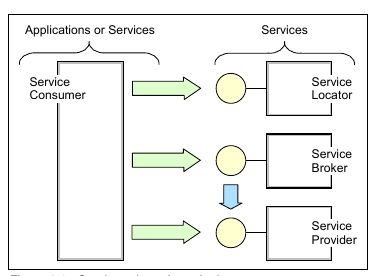
\includegraphics[width=0.80\textwidth]{img/7.png}
\caption{Plan de trabajo estándar del Conceptos esenciales de la Arquitectura Orientada a Servicios y la relación entre ellos
Fuente: Endrei et al. (2004)}
\label{figure:SOAworkflow}
\end{figure}

\section{Herramientas de software a utilizar}

Para la implementación del sistema se hizo uso de las siguientes herramientas de desarrollo web. Para la capa de interfaces de la aplicación, se utilizó Vue,js, un marco de trabajo desarrollado en JavaScript, que integra el etiquetado estándar de la web, así como soporte para estilos personalizados y lógica funcional. Por otra parte, del lado de la capa de datos, se desarrolló sobre Feathers.js, un marco de trabajo desarrollado enteramente en JavaScript que corre sobre el entorno de ejecución Node.js, que se comunica con una base de datos no relacional orientada a documentos MongoDB, mediante un mapeo objeto-documento a través de Mongoose. Finalmente, el lado del servidor fue desplegado en un entorno en la nube de Amazon Web Services, así como su entorno de desarrollo se encuentra alojado en MongoDB Atlas. A continuación, se mostrará a detalle cada herramienta utilizada para el desarrollo del producto final.

\subsection{Vue.js}

Vue (pronunciado /vjuː/, como view) \ref{figure:VueLogo} es un entorno de trabajo progresivo para desarrollar interfaces de usuario. Extraído de la página oficial del producto, ellos se describen a sí mismos de esta manera: “A diferencia de otros frameworks monolíticos, Vue está diseñado desde cero para ser utilizado incrementalmente. La librería central está enfocada solo en la capa de visualización, y es fácil de utilizar e integrar con otras librerías o proyectos existentes. Por otro lado, Vue también es perfectamente capaz de impulsar sofisticadas Single-Page Applications cuando se utiliza en combinación con herramientas modernas y librerías de apoyo”\cite{vuejs}.

\begin{figure}[H]
\centering

\includegraphics[width=0.80\textwidth]{img/8.png}
\caption{Logotipo de Vue.js
Fuente: https://vuejs.org/images/logo.png
Feathers}
\label{figure:VueLogo}
\end{figure}

\subsection{FeathersJS}

FeathersJS es un entorno de trabajo ligero utilizado para generar aplicaciones web de timepo real y APIs REST haciendo uso de JavaScript y TypeScript. Feathers en su núcleo es un conjunto de herramientas  que siguen una Arquitectura Orientada a Servicios, que permite construir prototipos y aplicaciones listas para ser desplegadas de manera rápida.

\begin{figure}[H]
\centering

\includegraphics[width=0.80\textwidth]{img/9.png}
\caption{Logotipo de Feathers.js
Fuente: https://feathersjs.com/img/feathers-logo-wide.png}
\label{figure:FeathersLogo}
\end{figure}

De manera general, una aplicación construida en Feathers se puede dividir en tres secciones: el lado del cliente (NodeJS) que representa el espacio de conexión de Feathers como una API, el lado del servidor que maneja los datos y la lógica de negocios, y el núcleo funcional, que es utilizado tanto en el cliente como en el servidor.

\subsection{MongoDB}

MongoDB \cite{mongodb} es un sistema de base de datos multiplataforma de esquema libre orientado a documentos que ofrece una gran escalabilidad y flexibilidad, así como un modelo de consultas e indexación avanzado. Dentro de sus conceptos elementales, están los siguientes:

\begin{description}
    \item[Base de datos:] Una base de datos es un contenedor físico para colecciones.
    \item[Colección:] Una colección es un grupo de documentos de MongoDB. Es el equivalente a una tabla en una base de datos relacional. Una colección existe en una base de datos individual. Las colecciones no fuerzan la existencia de un esquema.
    \item[Documento:] Un documento es un conjunto de pares de clave-valor. Los documentos tienen esquemas dinámicos. Un esquema dinámico implica que los documentos en la misma colección no necesariamente deben tener el mismo conjunto de campos o estructura.
\end{description}

\begin{figure}[H]
\centering

\includegraphics[width=0.80\textwidth]{img/10.png}
\caption{Logotipo de MongoDB
Fuente: https://www.agiliacenter.com/wp-content/uploads/2017/04/mongo-db-logo.png}
\label{figure:MongoDBLogo}
\end{figure}


\subsection{MongoDB Atlas}

MongoDB Atlas es un servicio de almacenamiento de datos en la nube proveído por MongoDB que permite alojar bases de datos no relacionales orientadas a documentos gestionados por MongoDB que pueden ser utilizadas por distintas aplicaciones web. Es reconocido por su flexibilidad y escalabilidad, así como por su tracción entre grandes compañías (7-Eleven, SEGA, Telefónica),  sus protocolos integrados de seguridad y el diseño particular orientado a aumentar la productividad de los desarrolladores \cite{mongodbAtlas}.

\subsection{AWS}

Amazon Web Services, también conocida como AWS, es un conjunto de herramientas y servicios de computación en la nube de Amazon. Este servicio se lanzó oficialmente en 2006 y para junio de 2007 AWS ya contaba con una base de usuarios de aproximadamente 180 mil personas. Entre las empresas que la utilizan se encuentran algunas como Reddit, Foursquare, Pinterest, Netflix, la NASA o la CIA.

\begin{figure}[H]
\centering

\includegraphics[width=0.80\textwidth]{img/11.png}
\caption{Logotipo de Amazon Web Services
Fuente: https://upload.wikimedia.org/wikipedia/commons/thumb/9/93/Amazon_Web_Services_Logo.svg/1200px-Amazon_Web_Services_Logo.svg.png}
\label{figure:AwsLogo}
\end{figure}

\subsection{Vercel}

Vercel es una plataforma en la nube para sitios estáticos y funciones sin servidor que se adapta perfectamente a su flujo de trabajo. Permite a los desarrolladores alojar sitios web y servicios web que se implementan instantáneamente, escalan automáticamente y no requieren supervisión, todo sin configuración \cite{vercel}.

\begin{figure}[H]
\centering

\includegraphics[width=0.80\textwidth]{img/12.png}
\caption{Logotipo de Vercel}
\label{figure:VercelLogo}
\end{figure}


\section{Infraestructura Propuesta}

La infraestructura a nivel de las herramientas propuestas en el esquema previo fue la explicada en la Figura \ref{figure:infraDiagram}.

\begin{figure}[H]
\centering
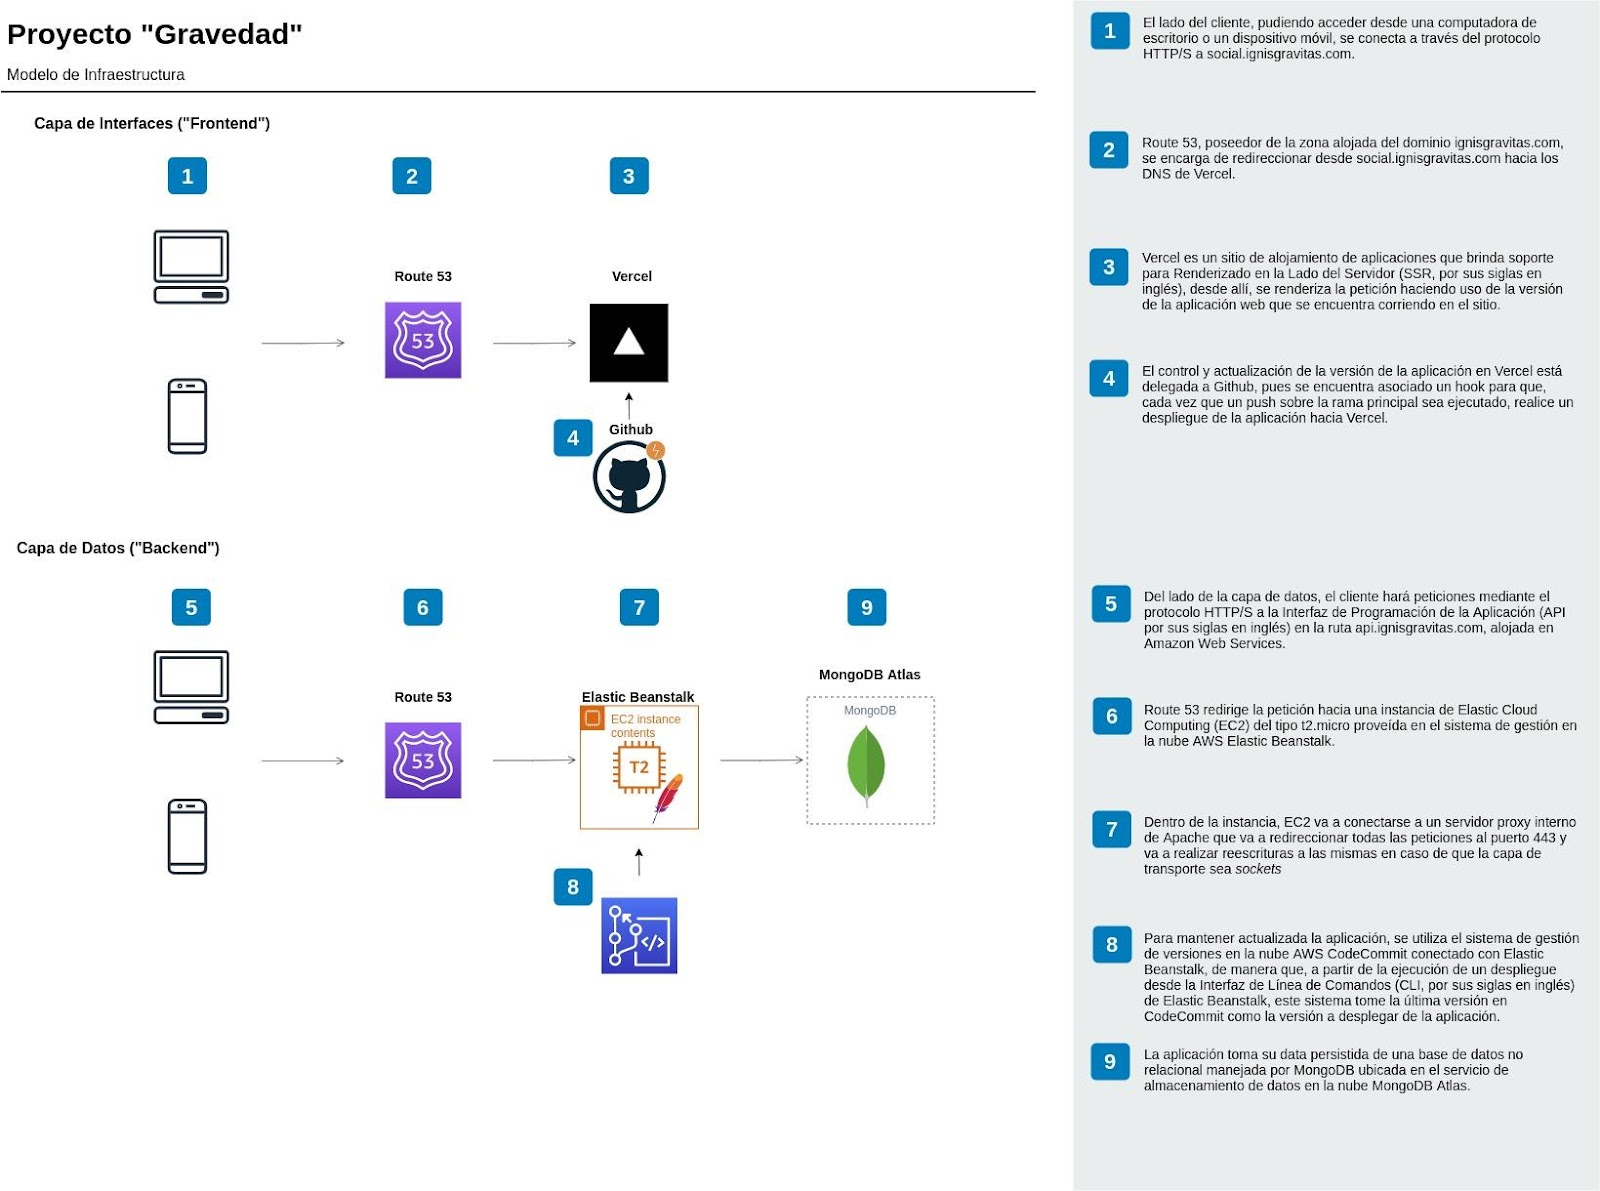
\includegraphics[width=0.80\textwidth]{img/13.jpg}
\caption{Infraestructura de capas del Proyecto “Gravedad”.
Fuente: Propia}
\label{figure:infraDiagram}
\end{figure}

Cada punto describe un elemento esencial dentro del sistema de funcionamiento de la aplicación.

\begin{enumerate}
    \item El lado del cliente, pudiendo acceder desde una computadora de escritorio o un dispositivo móvil, se conecta a través del protocolo HTTP/S a \texttt{social.ignisgravitas.com}.
    \item Route 53, poseedor de la zona alojada del dominio ignisgravitas.com, se encarga de redireccionar desde \texttt{social.ignisgravitas.com} hacia los DNS de Vercel.
    \item Vercel es un sitio de alojamiento de aplicaciones que brinda soporte para Renderizado en la Lado del Servidor (SSR, por sus siglas en inglés), desde allí, se renderiza la petición haciendo uso de la versión de la aplicación web que se encuentra corriendo en el sitio.
    \item El control y actualización de la versión de la aplicación en Vercel está delegada a Github, pues se encuentra asociado un hook para que, cada vez que un push sobre la rama principal sea ejecutado, realice un despliegue de la aplicación hacia Vercel.
    \item Del lado de la capa de datos, el cliente hará peticiones mediante el protocolo HTTP/S a la Interfaz de Programación de la Aplicación (API por sus siglas en inglés) en la ruta \textt{api.ignisgravitas.com}, alojada en Amazon Web Services.
    \item Route 53 redirige la petición hacia una instancia de Elastic Cloud Computing (EC2) del tipo t2.micro proveída en el sistema de gestión en la nube AWS Elastic Beanstalk.
    \item Dentro de la instancia, EC2 va a conectarse a un servidor proxy interno de Apache que va a redireccionar todas las peticiones al puerto 443 y va a realizar reescrituras a las mismas en caso de que la capa de transporte sea sockets.
    \item Para mantener actualizada la aplicación, se utiliza el sistema de gestión de versiones en la nube AWS CodeCommit conectado con Elastic Beanstalk, de manera que, a partir de la ejecución de un despliegue desde la Interfaz de Línea de Comandos (CLI, por sus siglas en inglés) de Elastic Beanstalk, este sistema tome la última versión en CodeCommit como la versión a desplegar de la aplicación.
    \item La aplicación toma su data persistente de una base de datos no relacional manejada por MongoDB ubicada en el servicio de almacenamiento de datos en la nube MongoDB Atlas.
\end{enumerate} % Descripción de arquitectura y tecnologías

Capítulo 6

En este capítulo se realizará un análisis sobre los resultados de la implementación a nivel de software de la arquitectura expuesta en el capítulo anterior.

Seguridad y Autenticación

Para el proceso de autenticación, se estableció el uso de dos métodos: el método clásico de correo electrónico y contraseña, y utilizando Open Authorization (de acá en adelante, referenciado como OAuth). Como se describe en el Diagrama 2,
Diagrama 2. Funcionamiento de Open Authorization en FeathersJS
Fuente: (Clusters, 2019)


Inicio de Sesión de la Plataforma
Fuente: Propia

Para la implementación manual del proceso de registro, se hizo uso de un proceso de confirmación a través de correo electrónico, como se muestra en la imagen siguiente:
Registro de usuarios. Fuente: Propia

Formulario Inicial de Usuario. Fuente: Propia
En dicho formulario se coloca la información mínima necesario para dar inicio al usuario dentro del sistema. Al ingresar estos datos, ya se encuentra posteriormente en la Vista Inicial:

Vista inicial de la plataforma Gravedad. Fuente: Propia

En esta vista se pueden apreciar las opciones para acceder a las distintas vistas y funcionalidades.
Botón desplegable de la barra de navegación superior.
Fuente: Propia

Al acceder a la opción para ver el Perfil de Usuario (Profile), se accede a la vista básica del usuario actual.

Usuarios

Si accedemos a la Vista de Edición de Usuarios, podemos contemplar los siguientes elementos:

Primera Impresión de la Vista de Usuarios. Fuente: Propia

En ella podemos ver las seis opciones referentes a la Información General del Usuario, su Educación, Experiencia Laboral, Habilidades, Preferencias como trabajador y su Cultura Individual.

En términos de la Información General, además de la selección estándar de fotografía de perfil, género, país y biografía, se plantea al usuario la selección de otra serie de opciones asociadas a las posiciones que tuvo el usuario previamente en términos laborales, así como la experiencia que posee, los roles preferidos y los roles primarios. Estos dos últimos selectores poseen una serie de opciones precargadas que le permitirán al usuario elegir su rol particular dentro de un conjunto de opciones limitado. Así mismo, se brinda la opción al usuario de introducir información relacionada con sus redes sociales y sitio web personal.

Información Gneeral del Perfil de Usuario. Fuente: Propia

Sección de Educación en el Perfil de Usuario. Fuente: Propia

En el plano de Educación, se desarrolló una lista dinámica a la cual el usuario puede agregar su experiencia académica a través del llenado de un formulario dentro de un modal. Este modal contiene información a introducir tal como: universidad a la que asistió para la titulación, fecha de graduación, grado obtenido y título obtenido.
Formulario para añadir nueva experiencia académica. Fuente: Propia
Sección de Experiencia Laboral. Fuente: Propia


Formulario de Experiencia Laboral. Fuente: Propia

En el plano laboral, al igual que en el de educación, se hizo uso de una lista dinámica para mostrar la experiencia académica del usuario. El modal que contiene el formulario solicita que se introduzca información referente a la compañía donde trabaja (o trabajó) el usuario, el cargo que ocupó allí, el inicio y final (si aplica) de su prestación de servicios y finalmente una descripción del trabajo realizado.

Con respecto a las Habilidades Laborales del Usaurio, se permite al usuario introducir habilidades dentro de una lista precargada, así como una breve descripción de sus logros y la posibilidad de cargar el curriculum.
Especificación de Habilidades Laborales. Fuente: Propia

Respecto a las preferencias laborales, la plataforma busca entender los gustos del trabajador y de cómo se siente cómodo trabajando, tanto en su ambiente actual como en términos de salario.
Preferencias Laborales I. Fuente: Propia

Preferencias Laborales II. Fuente: Propia

Dentro de las opciones para definir las opciones para definir la cultura del usuario, se destacan una serie de preguntas asociadas a las emociones que evoca el mismo como trabajador, por ejemplo la motivación interna del usuario, la proyección a largo plazo y una parametrización en términos de la cultura de la empresa a la que desea aspirar. Esto con el objetivo de encontrar el empleo ideal para este usuario en un futuro sistema de recomendaciones.

Cultura Laboral del Usuario I. Fuente: Propia
Cultura Laboral del Usuario II. Fuente: Propia
Finalmente, el perfil de usuario tiene la siguiente forma:
Perfil de usuario. Fuente: Propia

La vista de configuración de la cuenta, por su parte, únicamente tiene información básica, tal como el nombre y apellido, dirección correo electrónico, nombre de usuario y cambio de contraseña. Las demás opciones asociadas a privacidad, preferencias de cuenta e integraciones no se encuentran disponibles.
Menu de Configuración de Cuenta. Fuente: Propia

Publicaciones

Si deseamos crear una publicación, solo hace falta hacer click sobre la entrada de texto de “Crear un nuevo Post” en la sección central del menú inicial.

Espacio de creación de Posts. Fuente: Propia

Al realizar dicha acción, se va a desplegar un modal que muestra nuevamente una entrada de texto y otra serie de campos interactivos que permiten la inserción de imágenes y archivos. Allí se puede describir el contenido textual de la publicación, así como quién está realizando la publicación (si es una startup, un producto o un usuario) y las imágenes y contenido multimedia asociado.
Formulario para la creación de Publicaciones. Fuente: Propia

Al crearse una publicación, la misma es listada en tiempo real en la vista principal. La publicación también puede ser editada o eliminada dentro del menú en la parte superior de la publicación. Todas las publicaciones, al ser creadas, incluyen las siguientes funcionalidades:
La función de interacción “Me gusta”, para indicar apoyo a una publicación.
La función de comentar, que permite a los usuarios seguidores de otro usuario, startup o producto, emitir opiniones. También pueden editar o eliminar dichos comenarios.
La función de compartir publicación, para que dicha publicación sea listada también para los usuarios seguidores de cualquiera que comparta la publicación y no únicamente de quien la creó.
Publicación listada en la Vista Inicial. Fuente: Propia

Si el usuario clickea sobre la fecha y hora de la publicación, podrá ingresar a una vista dedicada donde únicamente tendrá la publicación presente. Esta vista dedicada puede ser compartida a través de un link, por si se desea llevar a un lugar externo a la plataforma. Todo usuario puede crear nuevos perfiles, tanto para una Startup como para un Producto.  Asímismo, se puede solicitar la posibilidad de ser inversor o de convertirse en un Aliado para que, manualmente, un desarrollador de Ignis Gravitas incorpore a dicho individuo al listado de inversores o aliados claves previa aprobación de la compañía Ignis Gravitas, Inc.

Menú desplegable para la creación de perfiles. Fuente: Propia

Startups	

Al seleccionar Crear Perfil de Startup, dicho usuario accederá a una vista de creación particular que se enfoca únicamente en la vista de las startups. Esta vista contiene una serie de secciones: Resumen, Personas, Cultura, Fondos y Trabajos.

Formulario de Creación de Startups. Fuente: Propia

Cada una de estas secciones contiene dentro de sí otra serie de datos de entrada. En la primera sección, se solicita la información básica de la startup, que se engloba en: Nombre de la Startup, dirección de correo electrónico, descripción básica de la startup, discurso de venta de la startup (pitch), país de origen, ciudad de origen, dirección física, dirección del sitio web de la startup, enlaces a las Redes Sociales de la startup, selección de los mercados a los cuales apunta la startup, enlace a un vídeo introductorio de la startup y, finalmente, historias de usuarios satisfechos con el trabajo de la startup.
Formulario de Información Básica de la Startup. Fuente: Propia

En la segunda vista, se pueden realizar las adiciones de membresías y hacer una descripción somera de lo que significa el equipo para la startup.

Formulario de la Sección Personas. Fuente: Propia

Al hacer click en el botón de agregar, se despliega un nuevo formulario que permite invitar nuevos miembros a la Startup. Estos nuevos miembros aparecerán luego en el perfil de la startup.

Formulario para añadir un nuevo miembro. Fuente: Propia

En la sección cultura, se añaden nuevas entradas de texto referentes a la descripción cultural de la startup, así como una serie de entrada de archivos para subir imágenes que muestren referencias a la compañía, como sus sitios de trabajo, personal, productos, etc. Además, se pueden agregar los beneficios y ventajas que ofrece la startup a cada uno de sus empleados.
Formulario de la Sección Cultura. Fuente: Propia

Añadir un nuevo beneficio. Fuente: Propia

En la sección de Financiamiento, se puede agregar la cantidad de dinero recibida hasta el momento, así como los inversores que han hecho contribuciones a la startup.

Entrada de datos de la sección Financiamiento. Fuente: Propia


Formulario para añadir un inversor. Fuente: Propia

En la sección de trabajos, se puede agregar la descripción general de la startup, así como las oportunidades de trabajo asociadas a la misma.

Entrada de datos en la sección Trabajo. Fuente: Propia
Formulario para propuestas de trabajo. Fuente: Propia
Productos

Al buscar crear un producto, se muestran el siguiente formulario:
El mismo, dividido en tres pestañas (“Resumen”, “Presentación” y “Personas”) permite detallar el producto ofertado. Los productos son, en una primera versión, independientes de las startups.
Sección Presentación. Fuente: Propia
Edición de Productos. Fuente: Propia
Menú General
Desde la Vista Principal, se pueden acceder a las distintas opciones de la plataforma:
Pila de Opciones de la Plataforma Gravitas. Fuente: Propia


Trabajos

El listado de trabajos es accesible desde la Pila de Opciones en el menú lateral. La misma posee la siguiente interfaz gráfica:

Vista de Listado de Trabajos

Del lado izquierdo, se ven las distintas ofertas de trabajo a las cuales puede aplicar un desarrollador, y a la derecha, una descripción detallada de la misma. Al hacer click sobre “Aplicar”, se muestra el siguiente formulario:
Formulario de aplicación a propuestas de trabajo. Fuente: Propia

Listado de Startups y Productos

Listado de Startup. Fuente: Propia

Al acceder al listado de startups, se puede contemplar cada una de las startups creadas por los distintos usuarios, así como aquellas sugeridas durante la selección del empleo previo, como un perfil creado por la comunidad y que no puede ser gestionado hasta no haber sido pedido y su autenticidad verificada.

Cada perfil contiene la información introducida en un principio de manera ordenada, así como los posts que ha publicado previamente:

Perfil de una startup. Fuente: Propia

En el listado de productos, por su parte, se ven los productos creados junto a su imagen, su nombre, su descripción básica, así como las etiquetas que lo describen. Así mismo, se tiene la posibilidad de votar al producto, para posicionarlo en la parte superior de la lista para los usuarios.
Lista de Productos. Fuente: Propia
Al acceder al perfil del producto, se puede ver toda la información introducida inicialmente para describir al mismo
Perfil de producto. Fuente: Propia

El resto de las vistas (“Invitaciones”, “Inversores”, “Mentores”, “Asesores” y “Aliados”) al momento de finalizar este proyecto no habían sido implementadas por lo que únicamente se replicó el mismo formato que en el listado de startups.

 % Descripcion de la plataforma funcional

\chapter{Conclusión y Recomendaciones}

\section{Conclusión}

El campo de la robótica es de suma importancia debido a la demanda para realizar tareas repetitivas, peligrosas, de alta precisión, la exploración del terreno, vigilancia, transporte de bienes y personas; todos estos campos y un sinnúmero más cuentan con un creciente soporte gracias a las investigaciones realizadas por universidades y grupos afines, al igual que empresas en el área comercial y militar, lo cual le hace merecedor de más estudio y desarrollo por parte de la Universidad de Los Andes, así como en nuestro país.

Es preciso entender que el desarrollo de software para robots está orientado al de plataformas de software debido a su capacidad de abstracción, modularización y amplio soporte por parte de comunidades de desarrolladores. Esto lo hace recomendable por encima del desarrollo de aplicaciones personalizadas para cada plataforma de hardware independiente.

Dentro de las plataformas de software consideradas, ROS es la mejor opción por la popularidad que cuenta en la comunidad de investigación y desarrollo robótico, el soporte al desarrollador a cualquier nivel entre novato a experto y la cantidad de módulos existentes para soportar distintos dispositivos o funcionalidades. No obstante, esto no significa que sea la única alternativa disponible, ya que otras plataformas son compatibles con ROS y pueden usarse en paralelo o sustituyéndola por completo.

Por otro lado, para fomentar el desarrollo de robots autónomos utilizando visión por computadora, es factible el uso de Kinect por su bajo costo (en especial al compararlo con sensores de medición láser) y facilidad de uso, a pesar de las limitaciones que pudiera tener, tales como rango y campo de visión limitado y la necesidad de poseer alimentación de corriente adecuada para el uso por parte de un robot móvil.

En lo que respecta al soporte del sistema operativo y de la plataforma de software elegida, contamos con distintos controladores, tales como freenect y openni, así como con alternativas de módulos para la generación de mapas de entorno utilizando Kinect, entre las que podemos nombrar hector\_slam, rgbdslam, RTAB-Map, etc., ya sea de forma individual o en conjunto con sensores láser y codificadores para la odometría. Si bien este proyecto se enfocó en la evaluación de un módulo particular, se tienen otras opciones ya mencionadas que podrían proveer de funcionalidades adicionales a las ya exploradas.

La generación del mapa de entorno se realizó mediante la elaboración a través de RTAB-Map de nubes de puntos provistas por el Kinect, por lo cual se comprobó su funcionamiento adecuado; de igual forma, se comprobó la coincidencia de la proyección 2D y el mapa de ocupación resultante con la detección de la nube de puntos.

Por último, es menester mencionar la utilidad de la aplicación de las metodologías Ágiles durante el desarrollo de este proyecto; éstas son por definición poco estrictas, en el sentido que permiten tomar o dejar de ellas lo que se requiera o no, por lo cual resultó factible y deseable tomar sencillamente algunos aspectos de cada método utilizado para, tal como el nombre indica, agilizar y facilitar el avance del proyecto sin que la aplicación del o de los métodos se convirtiese en una carga adicional para el estudiante o el profesor tutor.

\section{Recomendaciones}

Este proyecto tiene el potencial, si se quiere, de impulsar numerosos desarrollos en LaSDAI para la promoción, desarrollo e implementación de robots móviles autónomos. Por esto, se pueden realizar las siguientes recomendaciones:

\begin{itemize}
	\itemsep1pt \parskip1pt \parsep1pt
	\item Actualizar el sitio web de LaSDAI, incorporando las fuentes a los proyectos realizados y crear un repositorio de código público que los contenga.

	\item Agregar una \textit{wiki}, accesible públicamente, para colaboración de sus miembros.

	\item Continuar con el desarrollo del proyecto en al menos las siguientes áreas: integración del hardware de un robot móvil en ROS, detección de objetos o personas específicas utilizando OpenNI y Kinect.

	\item Proponer la implementación del desarrollo y control de proyectos en el laboratorio y/o en la escuela de sistemas utilizando Kanban y metodologías Ágiles, llevándolo inclusive al control de flujo de los distintos proyectos de grado dentro de la escuela.
\end{itemize}

\clearpage
\appendix
\renewcommand{\appendixname}{Apéndice}
\renewcommand{\appendixtocname}{Apéndices}
\renewcommand{\appendixpagename}{Apéndices}
\appendixpage
\noappendicestocpagenum
\addappheadtotoc
\chapter{Ignis Gravitas}

\section{Descripcion de Ignis Gravitas} \label{App:DescripcionLasdai}

Ignis Gravitas, Inc. es una startup registrada en Delaware, Estados Unidos. Su objetivo es expandir la cultura empresarial y el crecimiento de las startups en todo el mundo.

\subsection{Personal}

\subsubsection{Miembros}

\begin{itemize}
    \itemsep1pt \parskip0pt \parsep0pt
    \item Dr.\ Gerard Páez Monzón. (CEO)
    \item Br.\ Alfredo Ferreira Pace
    \item Br.\ Diego Benitez Peña
    \item Br.\ Aries Lugo
\end{itemize}

\subsection{Mision}

La misión de Ignis Gravitas, Inc. es la vinculación con el mundo emprendedor a través de la plataforma tecnológica y el segundo es la estructuración de una propuesta de valor complementaria como es la Academia Ignis Gravitas, donde se forman todos los interesados en el emprendimiento, con el objetivo de promover una nueva alternativa en la educación, adaptada a las nuevas demandas del mundo emprendedor.

\subsection{Vision}

Desde el punto de vista logístico y operativo, Ignis Gravitas tiene una personalidad enfocada a la aceleración de las diferentes Startups que surgen en su plataforma. Estos servicios se complementarán próximamente con los servicios de la Academia Ignis Gravitas, con el objetivo de aportar una visión integral en el desarrollo del proceso emprendedor al que se enfrentan las Startups en su día a día.


% Estilo de la bibliografía
\bibliographystyle{apa}
% Modificada ya que la original está en inglés.

% ***************************************************************** %
% Para agregar toda la bibliografia del archivo .bib
% solo descomente el siguiente comando
% ***************************************************************** %
\nocite{*}

% ***************************************************************** %
% Nombre del archivo con extensión .bib en donde se almacena la bibliografía
\bibliography{Referencias}

% ***************************************************************** %
% FIN DE
% Cuerpo
% ***************************************************************** %

\end{document}
